\documentclass[a4paper,12pt]{report}
\usepackage[utf8]{inputenc}
\usepackage[T1]{fontenc}
\usepackage[french]{babel} % If you write in French
\usepackage{a4wide}
\usepackage{graphicx}
\usepackage{placeins}
%pour la mise en page des tableaux
\usepackage{array}
\usepackage{tabularx}
\usepackage[table,xcdraw]{xcolor}
\usepackage{wrapfig}
\usepackage{color, colortbl}
\definecolor{Gray}{gray}{0.9}
\definecolor{LightCyan}{rgb}{0.88,1,1}
\usepackage{longtable}
\usepackage{float}
\usepackage{array} % for extrarowheight
\usepackage{lscape}
\usepackage{afterpage}
\usepackage{rotating}
\usepackage[nottoc,notlof,notlot]{tocbibind}
\usepackage{pdfpages}
\graphicspath{{images/}}
\usepackage{subfig}
\newlength\figureheight
\newlength\figurewidth
\usepackage{ifthen}
\usepackage{ifpdf}
\ifpdf
\usepackage[pdftex]{hyperref}
\else
\usepackage{hyperref}
\fi
\usepackage{color}
\hypersetup{%
	colorlinks=true,
	linkcolor=black,
	citecolor=black,
	urlcolor=blue}
% \urlstyle{same}

\usepackage{changepage}

\usepackage{multirow}

\setlength\arrayrulewidth{1pt}
\renewcommand{\baselinestretch}{1.05}
\usepackage{fancyhdr}
\pagestyle{fancy}
\fancyfoot{}
\fancyhead[LE,RO]{\bfseries\thepage}
\fancyhead[RE]{\bfseries\nouppercase{\leftmark}}




\setcounter{tocdepth}{5}
\setcounter{secnumdepth}{5}
\makeatletter
\newcounter {subsubsubsection}[subsubsection]
\renewcommand\thesubsubsubsection{\thesubsubsection .\@alph\c@subsubsubsection}
\newcommand\subsubsubsection{\@startsection{subsubsubsection}{4}{\z@}%
	{-3.25ex\@plus -1ex \@minus -.2ex}%
	{1.5ex \@plus .2ex}%
	{\normalfont\normalsize\bfseries}}
\newcommand*\l@subsubsubsection{\@dottedtocline{3}{10.0em}{4.1em}}
\newcommand*{\subsubsubsectionmark}[1]{}
\makeatother





\fancyhead[LO]{\bfseries\nouppercase{\rightmark}}
\setlength{\headheight}{14.5pt}

\let\headruleORIG\headrule
\renewcommand{\headrule}{\color{black} \headruleORIG}
\renewcommand{\headrulewidth}{1.0pt}
\usepackage{colortbl}
\arrayrulecolor{black}

\fancypagestyle{plain}{
	\fancyhead{}
	\fancyfoot[C]{\thepage}
	\renewcommand{\headrulewidth}{0pt}
}

\makeatletter
\def\@textbottom{\vskip \z@ \@plus 1pt}
\let\@texttop\relax
\makeatother

\makeatletter
\def\cleardoublepage{\clearpage\if@twoside \ifodd\c@page\else%
	\hbox{}%
	\thispagestyle{empty}%
	\newpage%
	\if@twocolumn\hbox{}\newpage\fi\fi\fi}
\makeatother

\usepackage{amsthm}
\usepackage{amssymb,amsmath,bbm}
\usepackage{array}
\usepackage{bm}
\usepackage{multirow}
\usepackage[footnote]{acronym}

\usepackage[bottom]{footmisc}

\newtheoremstyle{break}
{11pt}{11pt}%
{\itshape}{}%
{\bfseries}{}%
{\newline}{}%
\theoremstyle{break}
%\theoremstyle{definition}
\newtheorem{definition}{Définition}[chapter]

%\theoremstyle{definition}
\newtheorem{theoreme}{Théorème}[chapter]

%\theoremstyle{remark}
\newtheorem{remarque}{Remarque}[chapter]

%\theoremstyle{plain}
\newtheorem{propriete}{Propriété}[chapter]
\newtheorem{exemple}{Exemple}[chapter]

%table break line

\usepackage{multirow}



\usepackage{makecell}

\renewcommand\theadalign{bl}
\renewcommand\theadfont{\bfseries}
\renewcommand\cellalign{bl}
\renewcommand\cellgape{\Gape[2pt]}

\parskip=5pt
%\sloppy
 %%%%********************************************************************
\usepackage{xcolor}
\definecolor{quotemark}{gray}{0.7}
\makeatletter
\def\fquote{%
    \@ifnextchar[{\fquote@i}{\fquote@i[]}%] 
           }%
\def\fquote@i[#1]{%
    \def\tempa{#1}%
    \@ifnextchar[{\fquote@ii}{\fquote@ii[]}%]
                 }%
\def\fquote@ii[#1]{%
    \def\tempb{#1}%
    \@ifnextchar[{\fquote@iii}{\fquote@iii[]}%]
                      }%
\def\fquote@iii[#1]{%
    \def\tempc{#1}%
    \vspace{1em}%
    \noindent%
    \begin{list}{}{%
         \setlength{\leftmargin}{0.1\textwidth}%
         \setlength{\rightmargin}{0.1\textwidth}%
                  }%
         \item[]%
         \begin{picture}(0,0)%
         \put(-15,-5){\makebox(0,0){\scalebox{3}{\textcolor{quotemark}{``}}}}%
         \end{picture}%
         \begingroup\itshape}%
 %%%%********************************************************************
 \def\endfquote{%
 \endgroup\par%
 \makebox[0pt][l]{%
 \hspace{0.8\textwidth}%
 \begin{picture}(0,0)(0,0)%
 \put(15,15){\makebox(0,0){%
 \scalebox{3}{\color{quotemark}''}}}%
 \end{picture}}%
 \ifx\tempa\empty%
 \else%
    \ifx\tempc\empty%
       \hfill\rule{100pt}{0.5pt}\\\mbox{}\hfill\tempa,\ \emph{\tempb}%
   \else%
       \hfill\rule{100pt}{0.5pt}\\\mbox{}\hfill\tempa,\ \emph{\tempb},\ \tempc%
   \fi\fi\par%
   \vspace{0.5em}%
 \end{list}%
 }%
 \makeatother
 %%%%********************************************************************
 
 \frenchbsetup{StandardLists=true} % à inclure si on utilise \usepackage[french]{babel}
 \usepackage{enumitem}
 \usepackage{amssymb}
 \usepackage{afterpage}

\newcommand\blankpage{%
    \null
    \thispagestyle{empty}%
    \addtocounter{page}{-1}%
    \newpage}

\begin{document}

\begin{titlepage}
% \pagecolor{blue!10}
\begin{center}
	\begin{minipage}{2.5cm}
	\begin{center}
		
\includegraphics[width=2.5cm,height=1.7cm]{logo-ensak.png}
		
    \end{center}
\end{minipage}\hfill
\begin{minipage}{10cm}
	\begin{center}
	\textbf{ Université De Tunis El Manar}\\[0.1cm]
    \textbf{\uppercase{F}aculté des Sciences Economiques
    	et de Gestion de}\\[0.1cm]
    \textbf{-Tunis -}
\end{center}
\end{minipage}\hfill
\begin{minipage}{2.5cm}
	\begin{center}
	
\includegraphics[width=3.6cm,height=2.5cm]{uni.png}
	\end{center}

\end{minipage}
%
\includegraphics[width=0.6\textwidth]{logo-isae-supaero}\\[1cm]
\textsc{\Large }\\[1.5cm]
{\large \bfseries Rapport de  Projet de Fin d'\uppercase{é}tudes}\\[0.5cm]
{\large En vue de l'obtention du diplôme}\\[0.5cm]

%{\huge \bfseries \uppercase{Ingénieur d'état} \\[0.5cm] }
{\large \bfseries Licence Fondamentale en informatique de gestion}
\textsc{\Large }\\[0.5cm]

% Title
\rule{\linewidth}{0.3mm} \\[0.4cm]
{ \huge \bfseries\color{blue!70!black} Mise en place d'un système partagé et sécurisé
	dédié à l’enseignement à distance \\[0.3cm] }
\rule{\linewidth}{0.3mm} \\[0.4cm]
{\large \bfseries Réalisé au sein de l'Agence digitale N3RD}\\[0.4cm]
% 
\includegraphics[width=0.3\textwidth]{logo-isae-supaero}\\[1cm]
% Author and supervisor
 \noindent
\begin{minipage}{0.4\textwidth}
  \begin{flushleft} \large
    \emph{\color{orange!80!black}Réalisé par :}\\
    Khalfi Khawla,Kouki Hamza \\
    %\textsc{Khawla}
  \end{flushleft}
\end{minipage}%
\begin{minipage}{0.5\textwidth}
  \begin{flushright} \large
    \emph{\color{orange!80!black}Sous la direction de :} \\
    Pr.~Mohamed \textsc{Amnai} (ENSA)\\
    Pr.~Mohammed \textsc{Nasri} (ENSA)\\
    M\up{lle}.~Halima \textsc{Hadi} (SQLI)\\
    M. Faouzi \textsc{Amri} (SQLI)\\
  \end{flushright}
\end{minipage}\\[0.5cm]

\color{blue!80!black}{\large \textit{Soutenu le 01 juillet 2020, Devant le jury : }}\\[0.5cm]

\color{black}
\centering
\begin{tabular}{lll}
\large Pr.~Meriem \textsc{Mandar} : & \large ENSA Khouribga & \large - Présidente \\[0.1cm]
\large Pr.~Mohamed \textsc{Amnai} : & \large ENSA Khouribga & \large - Encadrant \\[0.1cm]
\large Pr.~Mohammed \textsc{Nasri} : & \large ENSA Khouribga & \large - Encadrant
\end{tabular}\\[0.7cm]

{\large \color{orange!80!black}{Année universitaire}\\ \color{blue!80!black}2019/2020}

\end{center}
\end{titlepage}

\chapter*{Dédicace}

\begin{fquote}
\begin{center}
\large{
Je dédie ce travail:\\[12pt]
\uppercase{à} ma chère mère et à mon cher père qui n'ont jamais cessé de me supporter, me soutenir et m'encourager durant mes années d'études et de moments de faiblesse et de maladie.\\[12pt]
Qu'ils trouvent ici le témoignage de ma profonde gratitude et reconnaissance.
\\[12pt]
\uppercase{à} mon frère et ma sœur qui me donnent de l'amour et de la vivacité.
\\[12pt]
\uppercase{à} mon binôme kouki hamza.
\uppercase{à} tous ceux qui m'ont aidé - de près ou de loin - ceux qui ont partagé avec moi les moments d'émotion lors de la réalisation de ce travail et qui m'ont chaleureusement supporté et encouragé tout au long de mon parcours.\\[12pt]
\uppercase{E}t Pour finir, à tous mes amis qui m'ont toujours encouragé.\\[12pt]
Merci!
}
\end{center}
\bigskip
\medskip
\end{fquote}

\begin{adjustwidth}{2cm}{1cm}
\hspace*{\fill} \textbf{\textit{\large{- Khawla}}}
\end{adjustwidth}

\clearpage
\chapter*{Dédicace}

\begin{fquote}
	\begin{center}
		\large{
			Je dédie ce travail:\\[12pt]
			\uppercase{à} ma chère mère, et à mon cher père ,Qui n'ont jamais cessé, de formuler des prières à mon égard, de me soutenir
			et de m'épauler pour que je puisse atteindre mes objectifs.
			\\[12pt]
			\uppercase{à} A mes frèresr Pour ses soutiens moral et leurs conseils précieux tout au long de mes études.
			\\[12pt]
			\uppercase{à}ma chère binôme ,Khalfi khawla, Pour leurs indéfectibles soutiens et leurs patiences infinies.
			\\[12pt]
			\uppercase{E}t tous ceux que j’aime et ceux qui m’aiment.\\[12pt]
			Merci!
		}
	\end{center}
	\bigskip
	\medskip
\end{fquote}

\begin{adjustwidth}{2cm}{1cm}
	\hspace*{\fill} \textbf{\textit{\large{- Hamza}}}
\end{adjustwidth}

\clearpage
\chapter*{Remerciements}

Nous adressons nos remerciements les plus sincères à  tous ceux qui de près ou de loin ont participé à la réalisation de ce travail. 

\medskip

Nous tenons à exprimer notre profonde gratitude, tout particulièrement,  à notre encadrant académique Monsieur \textbf{Mounir Nefzi} nous a fait profiter de ses larges connaissances et ses précieux conseils tout au long de ce travail. Il a toujours été à notre écoute et a su nous apporter un soutien sans faille.

\medskip


Nous souhaitons ensuite adresser nos remerciements au corps professoral et administratif de la Faculté de Sciences Economiques et de Gestion de Tunis, pour la qualité de l’enseignement offert et le soutien de l’équipe administrative.
\medskip

Nos Vifs remerciements sont adressés également, à notre maître de stage Monsieur \textbf{Ouesleti Nizar} et le directeur (à verfier) Monsieur \textbf{Bchini Tarek}  au sein de la Société d'Ingénierie et de Développement Web «N3RD» pour leurs accueils, le temps passé ensemble et le partage de leurs expertises . 
Nous saisissons également cette occasion pour adresser notre profond respect à toute l'équipe de travail qui ont fourni le cadre nécessaire pour la réalisation de notre projet.
.
\medskip

Pour finir, Nous voudrions adressons nos sincères remerciements aux membres du jury pour avoir bien voulu examiner et juger ce travail. \\[1cm]





\clearpage
%\chapter*{Résumé}

%Le présent rapport constitue une synthèse de mon projet de fin d'études effectué au sien de la société SQLI Rabat et ayant comme objectif la mise en œuvre d'une solution  PIM (Product Information Management) en faveur d'une maison de produits de luxe à base de la plateforme e-commerce SAP Hybris, et ce en vue de l’obtention du diplôme d'ingénieur d’état en informatique.

\medskip

%Ce projet vise à permettre à la société cliente qu'est une maison multinationale de vente des produits de luxe, de pouvoir gérer les informations relatives a ses produits d'une façon centralisée, afin de les utiliser dans plusieurs endroits, que ce soit au niveau de ses réseaux intranet et extranet ou pour alimenter les divers sites web, applications mobiles et points de vente qu'elle possède à travers le monde. Avec la solution proposée la société cliente peut exercer un contrôle de qualité et remédier au problèmes liés à la redondance et la non-cohérence des informations de ces produits qui peuvent être parfois assez critiques pour la réputation de l'entreprise vis-à-vis de ses partenaires et clients.

\medskip


%L’étude technique a été faite conjointement entre SQLI et la Maîtrise d’Ouvrage, vu l’expertise de SQLI dans les outils utilisés qui ont prouvé une efficacité inégale sur d’autre projets similaires. Durant ce stage, nous avons opté pour la méthodologie SCRUM pour la gestion et la conduite du projet.\\[1cm]

% \medskip

% La solution proposée a été construite en se basant sur la plate forme SAP Hybris vue son extensibilité étonnante et les éléments puissants qu'il fournit pour la gestion du contenu des produits d'une façon ergonomique et efficace Aussi que l'expertise de SQLI dans cette plateforme et les partenariats solides qu'a développé pour facilité son intégration pour ces clients.

%\noindent\rule[2pt]{\textwidth}{0.5pt}

%{\textbf{Mots clés :}}
%é-commerce, gestion de l'information produit, PIM, Java EE, SAP commerce, Hybris, SCRUM, SQLI.
%\\
%\noindent\rule[2pt]{\textwidth}{0.5pt}

%\clearpage
%\chapter*{Abstract}
%In order to get my degree in computer sciences, this report summarizes the work carried out within SQLI-Rabat Company for my graduation project, which consists of implementing and customizing a PIM (Product Information Management) solution for a luxury products company based on the SAP Hybris eCommerce platform.

%\medskip

%The project basically aims to enable the client company to manage their products information in a centralized way in order to be used in several places such as the extranet and the intranet, as well as in the different websites, mobile applications and selling points they have across the world. This will allow the company to control the quality of those information and avoid the problems resulting from their redundancy and non consistency, especially that they might be sometimes quite critical for the company to maintain a good reputation in front of its customers and partners.

% \medskip

% The technical study was made by SQLI in cooperation with the client, since SQLI gained a huge experience in the tools used which proved to be very effective, especially the SAP Hybrise platform due to its flexibility and the set of powerful features that it provides for the product content management or more commonly the PCM.

%\medskip

%The technical study was made by SQLI in cooperation with the client, since SQLI gained a huge experience in the tools used. The project was managed through an agile methodology which is SCRUM, in order to gain in flexibility and to better identify and respond to our client's needs.\\[1cm]

%\noindent\rule[2pt]{\textwidth}{0.5pt}

%{\textbf{Keywords :}}
%e-commerce, product information management, PIM, Java EE, SAP commerce, Hybris, SCRUM, SQLI.
%\\
%\noindent\rule[2pt]{\textwidth}{0.5pt}


%\clearpage
\tableofcontents
\clearpage
\listoffigures

\clearpage
\chapter*{Liste des sigles et acronymes}
\begin{acronym}[CP-OFDMX] % Give the longest acronym here

\acro{DAM}{\emph{Digital Asset Management}}
\medskip
\acro{ERP}{\emph{Enterprise Resource Planning}}
\medskip
\acro{EAI}{\emph{Enterprise Aplication Integration}}
\medskip
\acro{HAC}{\emph{Hybris Administration Console}}
\medskip

\acro{MEP}{\emph{Mise En Production}}
\medskip

\acro{OAT}{\emph{Operational Acceptence Testing}}
\medskip

\acro{OOTB}{\emph{Out Of The Box}}
\medskip

\acro{PIM}{\emph{Product Information Management}}
\medskip

\acro{PCM}{\emph{Product Content Management}}
\medskip

\acro{TFS}{\emph{Team Foundation Server}}
\medskip

\acro{UAT}{\emph{User Acceptence Testing}}
\medskip

\acro{WFJ}{\emph{Watches and Fine Jewelry }}
\end{acronym}

%%%%%%%%%%%%%%%%%%%%%%%%%%%%%%%%%%%%%%%%%%%%
%%% Content of the report and references %%%
%%%%%%%%%%%%%%%%%%%%%%%%%%%%%%%%%%%%%%%%%%%%

\cleardoublepage

\chapter*{Introduction générale}
\addcontentsline{toc}{chapter}{Introduction}
\markboth{Introduction}{Introduction}
\label{chap:introduction}
%\minitoc



\medskip

L’enseignement est un mode d’éducation permettant de développer les connaissances d’un
élève par le biais de la communication verbale et écrite. Il est centré sur le cours magistral.
\medskip

Les systèmes traditionnels d’enseignement imposent à tous les apprenants une unité de lieu,
une unité de temps, une unité d’action, une unité de rythme ce qui implique une rigidité des
mécanismes et une difficulté d’adéquation avec la réalité quotidienne. La tendance à l’amélioration du système sur le plan pédagogique par le recours aux moyens audiovisuels classiques
(projections de diapositives, de transparents, séquences vidéo) n’a pas résolu le problème. Il
existe en effet une solution de rechange à l’enseignement traditionnel. Cette forme d’enseignement relativement jeune, c’est la formation à distance qui permet d’acquérir des connaissances
et de développer des habiletés sans avoir à fréquenter un établissement d’enseignement et sans
la présence physique d’une personne qui enseigne. Dans ce cadre s’intègre notre projet de fin
d’étude qui est effectué au sein de la société N3RD. Notre objectif est de concevoir et mettre
en place un système partagé et sécurisé dédié à l’enseignement à distance.

\medskip

Ce rapport s’articulera donc, autour de quatre chapitres comme suit :
\medskip

Le premier chapitre permet de placer notre projet dans son contexte générale. Il comportera
une description de l’organisme d’accueil, exposera l’étude de l’existant, mettra l’accent sur la
solution proposée et abordera la méthode adoptée. Il présentera également quelques notions
théoriques importantes pour la réalisation de notre projet.

\medskip

Dans le deuxième chapitre, nous dégagerons les besoins les besoins fonctionnels et non fonctionnels, comme nous spécifierons un diagramme de cas d’utilisation général du produit avec le
langage de modélisation unifié UML.

\medskip

Le troisième chapitre elaborera l’étude conceptuelle de notre projet dont lequel nous allons
presenter quelues diagrammes.

\medskip

Le quatrième chapitre « La phase de clôture » sert à présenter l’ensemble des différents outils
utilisés pour concevoir et développer notre application ainsi que le diagramme de déploiement
et nous terminons par des captures d’écrans des principaux interfaces de l’application pour
illustrer la version finale de notre produit.

\medskip

Finalement, nous clôturerons ce rapport par une conclusion générale dans laquelle nous évaluerons le travail réalisé au sein de la société et nous proposerons des perspectives dans le but
d’améliorer notre travail.

\chapter{Contexte général du projet}
\label{chap:premierchapitre}

\begin{fquote}ce chapitre introductif est dans le but de mettre le travail dans son contexte général.
	Nous commençons tout d’abord par une présentation de l’entreprise d’accueil. Ensuite, nous
	mettons l’accent à décrire le sujet autour du quel se déroule notre projet de fin d’études. Enfin,
	nous allons faire la critique du système actuel et de proposer les solutions adéquats avant de
	mettre à disposition le langage et la méthodologie de conception.
 \end{fquote}

\clearpage
\section{Présentation de l’organisme d’accueil}

\subsection{Cadre général de travail}

\begin{figure}[hbt!]
  \centering
  
\includegraphics[width=5cm]{sqli_logo}
  \caption{Logo de la société N3RD.}
  \label{fig:logo-sqli}
\end{figure}
N3RD Créée en 2011 est une société d’ingénierie et de développement web qui, grâce à
l’utilisation des nouvelles technologies du web, est capable aujourd’hui d’assurer les différentes
tâches. \cite{wiki:sqli}.
\smallskip
\subsection{Domaines d’activité de l'entreprise}
N3RD est une société très active dans le domaine du développement Web et mobile ( sites
et applications), elle n’utilise que les dernières technologies :
\medskip
\begin{itemize}
  \item Web 2.0 et plus.
  \smallskip
  \item  Langages de développement côté serveur : PHP5, MySQL5, CSS3, HTML5
  \smallskip
  \item  Frameworks : Symphony2, Zend, Laravel et Code Igniter
  \smallskip
  \item CMSs : Prestashop, Drupal et WordPress.
  \smallskip
    \item Animation dynamique côté client : CSS3, JavaScript, Bootstrap, Ajax et JQuery.
  \smallskip
\end{itemize}
\medskip
\subsection{Mission de l'entreprise}
\begin{itemize}
	\item  Développement de sites et applications web pour tout business. 
	\smallskip
	\item Développement des solutions web personnalisées.
	\smallskip
	\item Conseils.
	\smallskip
	\item Boutiques en ligne et e-commerce.
	\smallskip
	\item Design sur mesure.
	\smallskip
	\item Création multimédia.
	\smallskip
	\item Infogérance (hébergement, gestion d’infrastructure...).
	\smallskip
	\item Création d’outils collaboratifs.
	\smallskip
	\item Optimisation pour les plateformes mobiles.
	\smallskip
	\item Création d’applications mobiles (Android IOS).
\end{itemize}

 

\section{Étude de l'existant}
\subsection{Cadre du projet}

Nous ne pouvons pas commencer ce travail sans avoir des informations et des idées claires et précises sur l’existant. L’étude de l’existant est une phase d’analyse qui consiste à faire un diagnostic sur les points forts et faibles du projet et déterminer des objectifs du nouveau système et l’ébauche de solution. Pour ce faire, il faut étudier le système existant lui même ainsi que l’environnement dans lequel il baigne.

\medskip
     
Après observation des plusieur site web université actuel nous avons constaté qu’il ne contient que les emplois du temps et les résultats en ligne ou quelques autres informations pour les etudiants(Stages..) .

\subsection{Problématique}
La formation à plusieur université se fait actuellement de façon traditionnelle (des enseignants, des étudiants et des cours sur place), et leur site ne contient ni des supports de cours ni des séries
d’exercices et n’offre pas la possibilité de passer les examens en ligne ce qui gêne les étudiants qui travaillent et veulent poursuivre leurs études en parallèle.
Alors notre mission est de résoudre
ce problème.

\subsection{Solution proposée}
En tenant compte des différents problèmes que nous avons évoqués, nous sommes amenés à
proposer une solution qui répond aux objectifs et qui pallie aux lacunes constatées aux niveau
de processus de l’existant.

 L’idée de notre projet consiste à mettre en place une application
web qui facilite l’étude à distance qui a pour principales missions de faciliter l’apprentissage
à distance en partageant les cours et les travaux dirigés entre l’étudiant et l’enseignant et en
permettant de passer les examens et d’avoir les notes et les résultats en ligne. 
\section{Planification et conduite du projet}
\subsection{Démarche adoptée}
Dans cette section, nous dévoilons le processus simplifié que nous préconisons pour la modélisation du système.
Nous présenterons également les principes fondamentaux du EXtreme Programming (XP) et
Scrum, afin d’éclairer les idées fortes auxquelles se rattache la démarche pratique adoptée dans
la suite du rapport.
	)
\begin{table} [!ht]
	\centering
	%	\centering
	\begin{tabular} { | m{5em} | m{7cm}| m{6cm} | }\hline
		\rowcolor[gray]{0.85}
		..... & Scrum &EXtreme Programming (XP) \\  \hline
		Description      & \small (La méthode s’appuie sur le découpage d’un
		projet en «sprint»,
		ainsi que l’autoorganisation de
		l’équipe de développement.
		Chaque sprint commence par une
		estimation suivie
		d’une planification
		opérationnelle.Le
		sprint se termine par
		une démonstration de
		ce qui a été achevé, et
		contribue à augmenter
		la valeur d’affaires du
		produit.)
		& \small (Ensemble de «Best
		Practices » de développement (Idéal pour
		le travail en groupe).
		- Cible des projets
		de moins de dix personnes.    \\    \hline
		Points forts )     &-Amélioration de la
		communication.
		-Règles définies clairement.
		-Augmentation de
		productivité.
		& -Simple à mettre en
		œuvre.
		-Fait une large place
		aux aspects techniques :prototypes,
		règles de développement, tests. . .  \\    \hline
		Points faibles    &  - Violation de responsabilité.
		-L’équipe ne se prete
		pas au SCRUM.&\small (- Ne couvre pas les
		phases en amont et
		en aval au développement : capture des besoins, support, maintenance, tests d’intégration. . .
		-Assez flou dans sa
		mise en œuvre.)   \\    \hline	
		
	\end{tabular}
	\caption{ Etude comparative entre les approches agiles}\label{tab: first-table}	
\end{table}

\clearpage
\subsubsection{presentation de la methode Scrum }
Scrum : Aujourd’hui « Scrum » est la méthode agile la plus populaire. Ce terme signifie «
mêlée » au rugby. La méthode scrum s’appuie sur des « sprints » qui sont des espaces temps
assez courts pouvant aller de quelques heures jusqu’à un mois. Généralement et de préférence
un sprint s’étend sur deux semaines. À la fin de chaque sprint, l’équipe présente ce qu’elle a
ajouté au produit.
\subsubsection{Processus de développement}
La nature du projet et sa forte dépendance aux acteurs du domaine sont les raisons qui expliquent le fait d’être toujours à l’écoute du client et prêt à répondre à ses nouveaux besoins. C’est pour cela, l’équipe du projet a opté pour un cycle de développement agile et plus précisément SCRUM.

\medskip

Le principe de la méthodologie SCRUM est de développer un logiciel de manière incrémentale en maintenant une liste totalement transparente des demandes d'évolutions ou de corrections à implémenter (backlog).

\medskip

Avec des livraisons très fréquentes, toutes les 4 semaines en général, le client reçoit un logiciel à chaque itération. Plus nous avançons dans le projet, plus le logiciel est complet et possède de plus en plus de fonctionnalités.

\medskip

Pour cela, la méthode s'appuie sur des développements itératifs à un rythme constant d'une durée de 2 à 4 semaines (2 semaines pour notre cas) comme le montre la figure \ref{fig:scrum} :

\begin{figure}[ht]
  \centering
  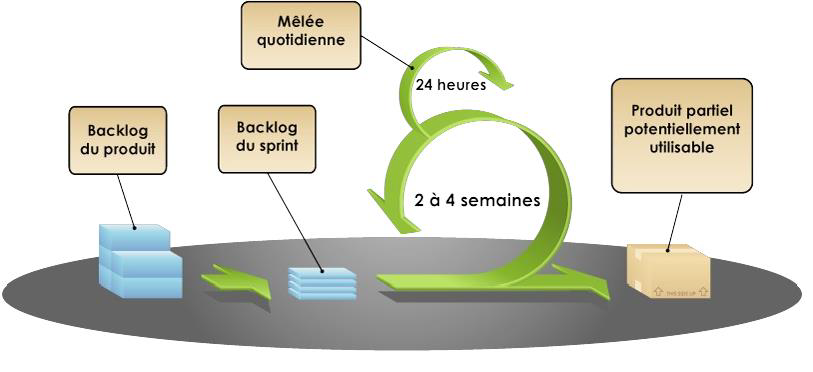
\includegraphics[width=15cm,height=6.2cm]{scrum}
  \caption{Cycle de vie de la méthodologie scrum.}
  \label{fig:scrum}
\end{figure}
\FloatBarrier

Le schéma illustre un exemple de planification en Scrum : les itérations (sprints) durent en pratique entre 2 et 4 semaines, et possède chacune un but. Le but de chaque sprint une liste d'items du backlog de produit ou de fonctionnalités à réaliser. Ces items sont décomposés par l'équipe en tâches élémentaires de quelques heures.

\medskip

Comme nous pouvons le remarquer dans cette figure, pour mettre en place la méthode SCRUM, il faut tout d'abord définir les différentes fonctionnalités de notre application qui forment le backlog du produit. Ensuite, vient l'étape de la planification du sprint pour définir le plan détaillé d'une itération.

\medskip

Durant un sprint, il y a toujours des réunions quotidiennes entre les différents collaborateurs du projet afin de présenter l'état d'avancement des différentes tâches en cours, les difficultés rencontrées ainsi que les tâches restantes à réaliser. Une fois le produit partiel est prêt, nous vérifions la conformité de ce qui a été fait durant le sprint et nous pouvons alors l'améliorer en procédant à l'étape de rétrospective.

\medskip
\subsubsection{l'equipe Scrum}
Scrum est considéré comme un cadre ou un «framework» de gestion de projet. Ce cadre est
constitué d’une définition des rôles, il s’articule autour des trois rôles qui sont principalement les suivants :

\medskip

\begin{itemize}
  \item \textbf{Product Owner} :\small ( Dans la majorité des projets, le responsable produit (product owner) est le responsable de l'équipe projet client. C'est lui qui va définir et prioriser la liste des fonctionnalités du produit et choisir la date et le contenu de chaque sprint sur la base des valeurs (charges) qui lui sont communiquées par l'équipe.)
  \smallskip
  \item \textbf{ScrumMaster} : Véritable facilitateur sur le projet, il veille à ce que chacun puisse travailler au maximum de ses capacités en éliminant les obstacles et en protégeant l'équipe des perturbations extérieures.
  \smallskip
  \item \textbf{Équipe de dévelopement} : elle regroupe l’ensemble des rôles habituellement nécessaires à un projet, à savoir le concepteur, le développeur, le testeur, etc. L'équipe s'organise elle-même et elle reste inchangée pendant toute la durée d'un sprint.

\textbf{Dans notre cas, les rôles sont répartis comme suit :}

\end{itemize}

\begin{table} [!ht]
	\centering
	\begin{tabular} {|c|c|}\hline
		Rôle & Personne \\  \hline
		Product owner     & La société N3RD      \\    \hline
		Scrum Master     & Mr Ousleti nizar    \\    \hline
		Équipe de développement    &  Mr kouki hamza ,
		Mlle khalfi khawla     \\    \hline	
		
	\end{tabular}
	\caption{Equipe Scrum}\label{tab: first-table}	
\end{table}
\clearpage
\subsubsection{les événements Scrum}
Dans le cadre du scrum, il y a 05 événements pour créer de la régularité et minimiser le besoin de rencontres. Tous les événements sont classés dans le temps (time-boxed), ce qui signifie que ces événements ont une durée maximale.
\begin{itemize}[label=$\square$,leftmargin=* ,parsep=0cm,itemsep=0cm,topsep=0cm]
	\item \textsf{Sprint:} c’est le cœur du scrum. Un sprint est lorsqu’un incrément de produit est créé. Un incrément est une partie utilisable et potentiellement fonctionnelle du produit final. Les sprints sont classés dans le temps pour un mois ou moins. Chaque sprint a un objectif de ce qui doit être construit. 
	\item \textsf{La planification du sprint (Sprint planning)} est l’événement où l’équipe scrum définit ce qui sera livré dans un sprint. Cet événement est limité dans le temps à un maximum de huit heures pour un sprint d’un mois. Dans la planification du sprint, l’équipe scrum définira ce qui peut être livré au prochain incrément et combien de travail est nécessaire pour atteindre cet objectif. L’entrée principale de cette réunion est le Product Backlog où le Product Owner et le DevTeam choisiront les éléments qui seront inclus dans ce sprint pour atteindre l’objectif du sprint. 
	\item \textsf{Le Daily scrum} est une réunion quotidienne de 15 minutes pour DevTeam où ils mettront à jour le statut de travail et les plans pour les prochaines 24 heures. Cette réunion est utilisée pour inspecter l’état d’avancement du sprint. Lors de cette réunion, chaque membre du DevTeam répondra aux questions suivantes:
	\begin{enumerate}
		\item Qu’est-ce qui a été accompli depuis la dernière réunion?
		\item Que fera-t-on avant la prochaine rencontre?
		\item Voyez-vous un obstacle qui vous empêche, ou le DevTeam, d’atteindre l’objectif de sprint?
	\end{enumerate}
	\item \textsf{La revue de sprint (Sprint review)} est utilisée par l’équipe scrum pour présenter et inspecter l’incrémentation à la fin d’un sprint. Il est limité à quatre heures pour un sprint d’un mois. Cette réunion est destinée à obtenir des commentaires et des demandes de changement du client et des parties prenantes. Seuls les éléments considérés comme « terminés (Done)» sont inclus dans la revue de sprint. 
	\item \textsf{La rétrospective Sprint (Sprint retrospective)} est un événement destiné à traiter l’amélioration. Les améliorations pourraient concerner les personnes, les relations, les processus et les outils. Il faut trois heures pour un sprint d’un mois. 
\end{itemize}

\subsection{Planning du projet}

La planification du projet est une phase importante d’avant-projet. Elle consiste à prévoir le déroulement de ce dernier tout au long des phases constituant le cycle de développement.

\medskip
\begin{itemize}
\item[$\bullet$] \textbf{Le diagramme de Gantt:}

Le diagramme de Gantt, couramment utilisé en gestion de projet, est l'un des outils les plus
efficaces pour représenter visuellement l'état d'avancement des différentes activités (tâches) qui constituent un projet.
Ce diagramme permet donc de visualiser d'un seul coup d'œil :
  \begin{itemize}
	\item[$\star$]Les différentes tâches à envisager. 
	\item[$\star$]La date de début et la date de fin de chaque tâche.
	\item[$\star$] La durée escomptée de chaque tâche. 
	\item[$\star$] Le chevauchement éventuel des tâches, et la durée de ce chevauchement.
	\item[$\star$] La date de début et la date de fin du projet dans son ensemble.
\end{itemize}





















Le diagramme de Gantt dans la figure \ref{fig:gantt} illustre le déroulement du stage dans le temps:
\end{itemize}

%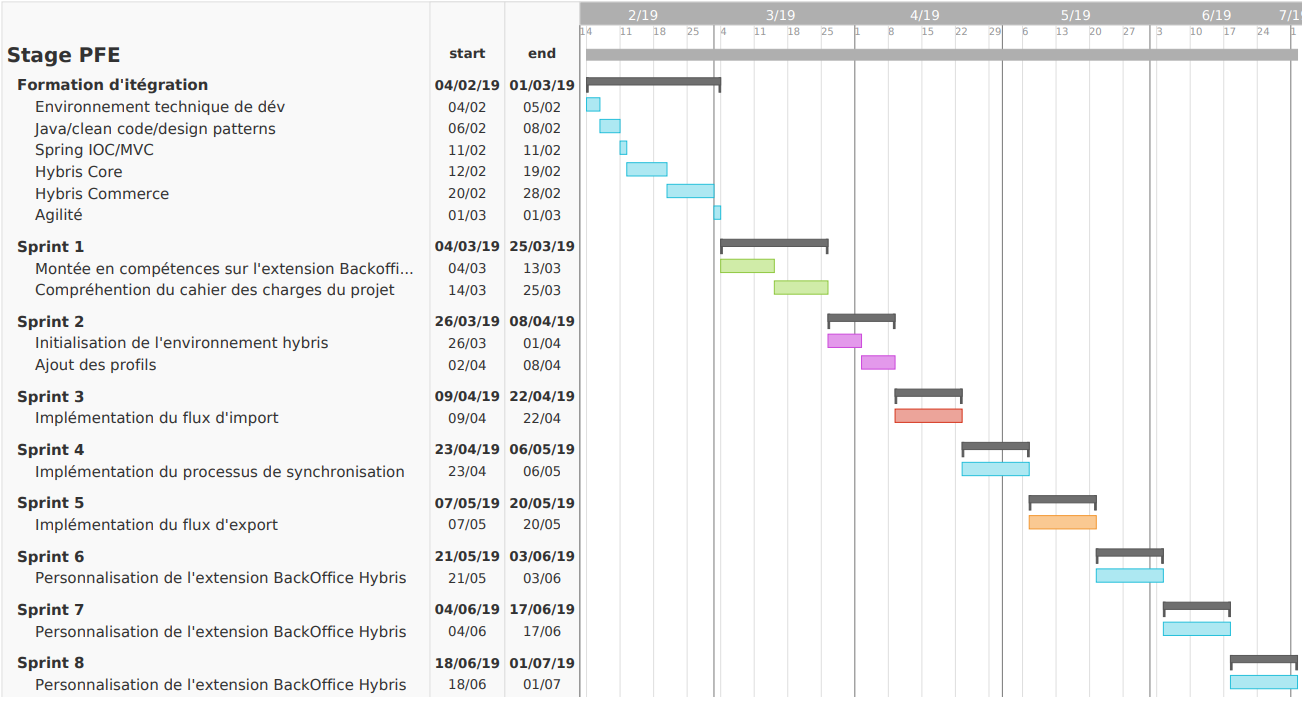
\includepdf[pages=-]{gantt.pdf}
\begin{figure}[ht]
  \centering
  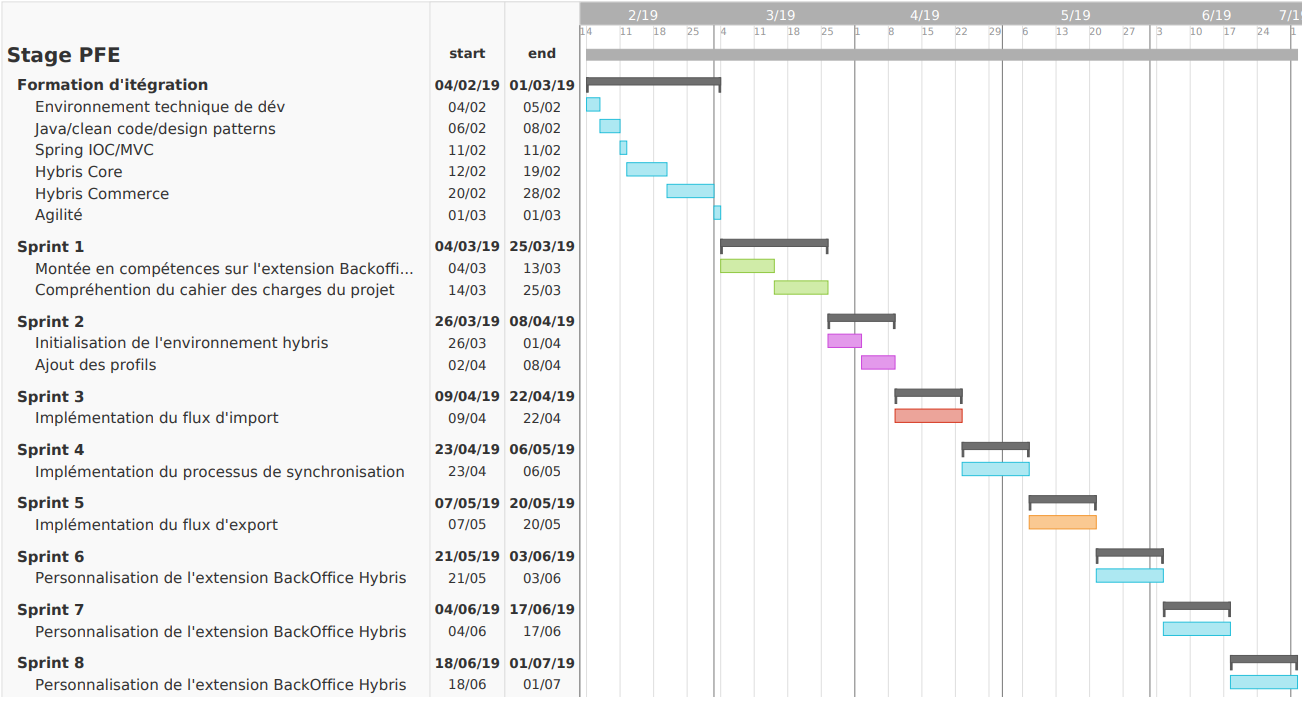
\includegraphics[height=14cm,width=16cm,angle=-90,origin=c]{gantt.PNG}
  \caption{Diagramme de gantt du projet.}
  \label{fig:gantt}
\end{figure}
\clearpage
\FloatBarrier
\subsection{La modélisation objet}
Depuis quelques années, la modélisation objet avec le langage UML est devenue une pratique
courante sur de nombreux projets informatiques. En effet, Le recours à la modélisation est
une pratique indispensable au développement logiciel, car un modèle est prévu pour arriver à
anticiper les résultats du codage.
\subsubsection{Définition de UML}
UML se définit comme un langage de modélisation graphique et textuel destiné à comprendre et décrire des besoins, spécifier et documenter des systèmes, esquisser des architectures
logicielles, concevoir des solutions et communiquer des points de vue. UML unifie à la fois les
notations et les concepts orientés objet. Il ne s’agit pas d’une simple notation graphique, car
les concepts transmis par un diagramme ont une sémantique précise.
UML s’articule autour de treize types de diagrammes, chacun d’eux étant dédié à la représentation des concepts particuliers d’un système logiciel [3].


\subsubsection{Processus de modélisation}
Le processus que nous allons présenter et appliquer tout au long de ce rapport :

\begin{itemize}
	\item Conduit par les cas d’utilisation ;
	\item Relativement léger et restreint, comme les méthodes agiles, mais sans négliger les activités
	de modélisation en analyse et conception ;
	\item Fondé sur l’utilisation d’un sous-ensemble nécessaire et suffisant du langage UML, conformément à méthodes agiles.
\end{itemize}



\section{Conclusion}

Tout au long de ce chapitre, nous avons décrit l’organisme d’accueil , nous avons aussi
formulé une petite présentation de notre projet pour vous mettre en contexte. Nous avons
ensuite fait une étude de l’existant dans l’entreprise pour pouvoir dégager les différentes lacunesainsi que les solutions envisagées. A la fin de ce chapitre, nous avons dévoilé le langage et laméthodologie de conception de notre système.
Le chapitre suivant sera consacré à la planification du projet ainsi que la spécification des
besoins

\chapter{Analyse et spécification des besoins}
\label{sec:unchapitre}

\begin{fquote}Dans ce chapitre, j’aborde les phases d’analyse et de spécification des besoins du projet, dans le but d’avoir une vision globale claire du comportement du projet ainsi que les attentes des utilisateurs.
 \end{fquote}
\begin{figure}[ht]
	\centering
	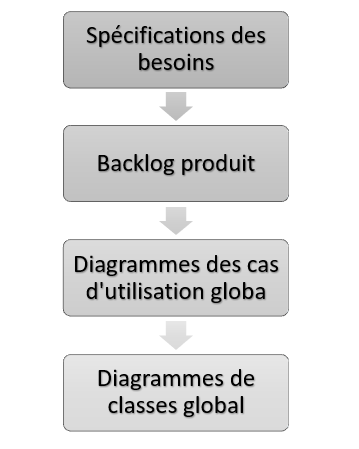
\includegraphics[width=8cm,height=9cm]{Sanstllitre2.png}
	\caption{Section de chapitre 2.}
	\label{fig:Section de chapitre 2}
\end{figure}
\FloatBarrier
\clearpage

\section{Spécifications des besoins}

La spécification des besoins va nous permettre d’avoir une meilleure approche des utilisateurs, des fonctionnalités et de la relation entre les deux. Elle sera sous forme de besoins. Pour cela nous allons procéder comme ceci :
\begin{itemize}
	\item Identification des acteurs du nouveau système.
	\item Identification des besoins fonctionnels.
	\item Identification des besoins non fonctionnels .
\end{itemize}

\subsection{Le processus d’apprentissage}

\begin{itemize}
	\item \underline{Apprentissage }: L’apprentissage est décrit comme un ensemble de mécanismes menant à
	l’acquisition de savoir, savoir -faire, savoir-être ou de connaissances.
	Dans ce processus l’acteur de l’apprentissage est appelé apprenant son rôle et d’acquérir la
	connaissance qui peut être opposé à l’enseignement dont le but est de dispenser des connaissances
	et savoirs. 
	
	
	\item  \underline{ Enseignement} : L’enseignement est l’action de transmettre des connaissances nouvelles ou
	savoirs à un apprenant (instruire et endoctriner tout en respectant certaines règles). Il s’agit du
	système et de la méthode d’enseigner, composée par tout un ensemble de connaissances, de
	principes et d’idées transmis à quelqu’un.
	L’enseignement constitue un composant de l’éducation, ce dernier terme beaucoup plus
	général, correspond à la formation globale d’un individu, à divers niveaux (au niveau religieux, moral,
	social, technique, scientifique, médical, etc.) 	
	\item \underline{ Didactique }: La didactique vient du grec qui signifie "enseigner", c’est la science qui a pour
	objet l’étude des méthodes et des pratiques de l’enseignement en général, ou de l’enseignement
	d’une discipline ou d’une matière particulière .
	Une méthode didactique c’est une méthode d’enseignement qui suit une approche
	scientifique ou style éducatif cohérente pour engager l’esprit de l’étudiant. Et on distingue :
	\begin{itemize}	
	\item[$\star$] La didactique générale qui s’intéresse à la conduite de la classe (cours magistraux,
	leçons dialoguées, travaux pratiques individuels ou collectifs, utilisation de manuels,
	etc.);
	\item[$\star$] La didactique spéciale qui s’intéresse à l’enseignement d’une discipline particulière
	pour une classe, un cycle d’études ou un ordre d’enseignement.
\end{itemize}
	\item \underline{ Le triangle didactique }: proposé par Jean Houssaye en 1988 comme modèle de
	compréhension du pédagogique. Il se compose des composantes principales d’un acte pédagogique
	(étudiant, savoir, enseignant) et les processus (apprendre, enseigner, former). De cela, il permet de faire des comparaisons entre les diverses situations pédagogiques  :
	\begin{figure}[ht]
		\centering
		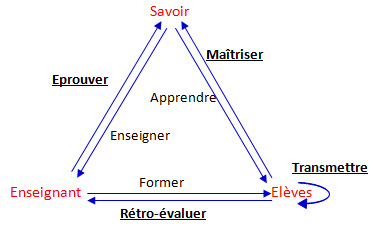
\includegraphics[width=14cm,height=10cm]{LetriangledejeanHoussaye.jpg}
		\caption{ Le triangle de jean Houssaye.}
		\label{fig: Le triangle de jean Houssaye}
	\end{figure}
	\FloatBarrier
	
	
		\begin{itemize}	
		\item[$\star$] Le processus Enseigner : axé de façon privilégiée sur la relation Savoir-Enseignant, et sur
		la transmission de ce savoir structurée par l’enseignant.
		\item[$\star$] Le processus Former : axé sur la liaison Enseignant-Former. Il correspond aux pédagogies
		centrées sur la formation humaine et sur la socialisation.
     	\item[$\star$]Le processus Apprendre : Il porte sur le rapport direct Savoir-Apprenant. Là, l’enseignant
    	devient l’organisateur de situations et de conditions externes d’apprentissage par
    	lesquelles il met en relation savoir et apprenant en jouant un rôle de médiateur.
	
     \end{itemize}
\end{itemize}







\clearpage

\subsection{Identification des acteurs}
Un acteur est une personne, un matériel ou un logiciel qui interagit avec le système. L’analyse du présent projet commence par une identification des acteurs agissants sur les différentes parties du système. Les acteurs présentés dans la figure \ref{fig:profiles} sont des employés du clients en plus du serveur  qui est la solution adoptée par le client pour la communication et le partage des informations entre ces systèmes et départements .

\begin{figure}[ht]
  \centering
  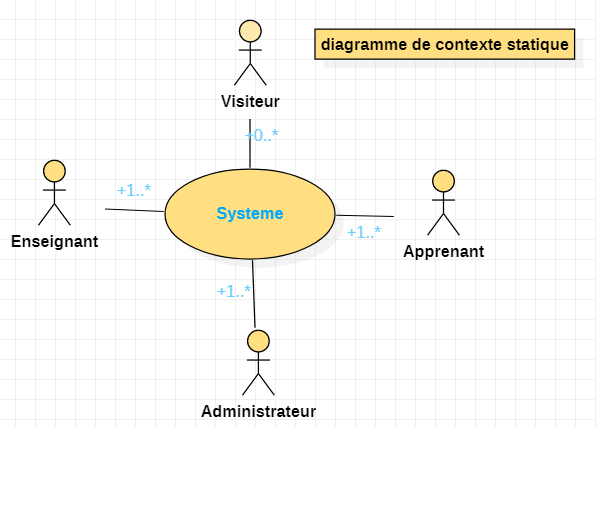
\includegraphics[width=14cm,height=8.5cm]{profiles}
  \caption{Héirarchie des profiles humaines.}
  \label{fig:profiles}
\end{figure}
\FloatBarrier
Le tableau \ref{actors} récapitule les acteurs en interaction avec le système en spécifiant le rôle de chacun avant de définir plus précisément leurs interactions avec le système en utilisant des diagrammes de cas d'utilisation.\\

\begin{table}[H]
\centering
\def\arraystretch{1.45}
\begin{tabular}{|c|c|}
\hline
\rowcolor{Gray} 
Acteur           & Fonction                                                                                                                                                                                                                                             \\ \hline
\rowcolor{LightCyan} 
Administrateur    & \begin{tabular}[c]{@{}c@{}} L’administrateur est la personne responsable de gérer la totalité du système.\\  \end{tabular} \\ \hline
\rowcolor{LightCyan} 



Enseignant & \begin{tabular}[c]{@{}c@{}} C’est un acteur principale qui interagit avec notre application.\\
C’est l’acteur qui a pour rôle de gérer les cours,\\ les travaux dirigés (TD) et les examens des
étudiants.\end{tabular}                   \\ \hline
\rowcolor{LightCyan} 



 
Apprenant & \begin{tabular}[c]{@{}c@{}}L’apprenant inscrit, il va pouvoir consulter \\les cours et faire les tests qui lui sont
	proposés.\\ L'apprenant peut avoir la possibilité de participer aux forums,\\ d'envoyer un
	message à un tuteur, \\à un autre apprenant ou même à l'administrateur.\\ Ainsi la possibilité
	de discussion en ligne avec le tuteur,\\ la modification de son profil et la consultation de
	sesrésultats.\end{tabular}                   \\ \hline
\rowcolor{LightCyan} 



Visiteur & \begin{tabular}[c]{@{}c@{}}N’importe quel visiteur qui \\veut télécharger des cours via un compte personnelle a
	condition \\ de faire les inscriptions pour avoir un compte.\end{tabular}                   \\ \hline
\rowcolor{LightCyan} 
\end{tabular}
\caption{Acteurs en interaction avec le système}
\label{actors}
\end{table}

\subsection{Les besoins fonctionnels}
Les besoins fonctionnels expriment une action que doit effectuer le système en réponse à une demande .\\
Les besoins principaux à couvrir par le système sont les suivants :\\
{\color{cyan} Si l’acteur est un Administrateur, il peut :
}

\begin{itemize}
	\item \underline{S’authentifier}  :l’Administarateur entre son « username » et son « password » avant d’accéder à l’application pour assurer la confidentialité des informations.
	\item \underline{Gérer les comptes des utilisateurs} : l’Administrateur peut ajouter des comptes pour les
	nouveaux Utilisateurs(Enseignant ou Etudiant) , modifier leurs informations et supprimer
	les comptes des anciens utilisateurs.
\end{itemize}
\clearpage
{\color{cyan}Si l’acteur est un Enseignant, il peut :}
\begin{itemize}
	\item \underline{Gérer les Matières} :l’Enseignant peut ajouter, modifier et supprimer les matières.
	\item  \underline{Gérer les Cours }:l’Enseignant peut ajouter, modifier et supprimer les cours.

	\item \underline{Gérer les Traveaux dirigés(TD) }:l’Enseignant peut ajouter,modifier et supprimer les Traveaux dirigés(TD).
	\item \underline{Gérer les Examens }:l’Enseignant peut ajouter des examens en choisissant une durée de
	temps determiné.
\end{itemize}
{\color{cyan}Si l’acteur est un Etudiant, il peut :}
\begin{itemize}
	\item \underline{Consulter les Cours} :l’Etudiant peut consulter et télecharger les cours.
	\item \underline{Consulter les Traveaux dirigés(TD) }:l’Etudiant peut consulter et télecharger les Traveaux
	dirigés(TD).
	\item \underline{Passer les Examens }:l’Etudiant peut passer les examens en respectant une durée de temps
	determinée.
\end{itemize}

\subsection{Les besoins non fonctionnels}
Les besoins non fonctionnels impressionne directement sur déroulement réelle de l’application. Ce sont des besoins techniques décrivant la majorité des contraintes (qu’on a déjà
approuvée dans le chapitre précèdent) auxquelles est soumis le système pour sa réalisation et
son bon fonctionnement. Pour cela l’ensemble des extensions à réaliser doivent respecter les besoins suivants :
%Les besoins non fonctionnels représentent les exigences implicites auquel le système doit répondre. Parmi ces besoins on cite :

\begin{itemize}
	\item \underline{La Sécurité} : La solution proposée permet à l’utilisateur une navigation sécurisée.
	Elle n’est accessible qu’avec une authentification.
	\item \underline{Ergonomie de l’interface }: L’ergonomie est un élément important de l’application : les
	écrans de saisie doivent être clairs, organisés avec cohérence, de façon à ce qu’une prise
	en main soit la plus rapide possible.
	\item \underline{
Maintenance }: L’une des plus importantes besoins de notre application est la facilité de
	modification pour s’adopter aux nouveaux besoins.
	\item \underline{Portabilité} : L’application doit être accessible via n’importe quel navigateur.

\end{itemize}

%\section{Analyse des besoins fonctionnels}
%L’analyse des besoins est une étape très importante dans le processus de l’étude et le développement des systèmes d’informations. Cette partie identifie l’ensemble des acteurs qui interagissent avec le système et définit l’ensemble des cas d’utilisation de ce dernier en se basant sur les diagrammes UML.
\section{Backlog produit}
Le Backlog produit est une liste ordonnée de tout ce qui pourrait être nécessaire dans un produit et constitue l’unique source d'exigences pour toutes les modifications apportées au produit. Le Product Owner est responsable du Backlog produit, y compris son contenu, sa disponibilité et son ordonnancement.\\
 Ses toutes premières moutures ne font qu’esquisser les besoins tels qu’initialement connus et compris. Le Backlog Produit évolue au fur et à mesure que le produit et le contexte dans lequel il sera utilisé évoluent. Le Backlog Produit est dynamique; il change constamment pour identifier ce que le produit requiert pour être approprié, compétitif et utile. Tant et aussi longtemps qu’un produit existe, son Backlog Produit correspondant existe.\\
 Les caractéristiques fonctionnelles sont appelées
 des histoires utilisateurs (user story). Les user stories sont caractérisés par :\\
\begin{itemize}[label=$\square$,leftmargin=* ,parsep=0cm,itemsep=0cm,topsep=0cm]
    \item \textit{\textbf{Identifiant}} Il détermine un identifiant unique pour l’histoire en question.\\
 	
 	\item \textit{\textbf{Description}}Elle décrit le besoin d’un acteur.\\
 	
 	\item \textit{\textbf{Critères d’acceptation}}À chaque user story sont associés des critères permettant au client
 	de tester l’histoire. Ces critères d’acceptation peuvent être formalisés, pour aller un peu plus
 	loin dans l’aide fournie à l’équipe que l’énoncé de ces critères.\\
 
 	\item \textit{\textbf{Estimation}}Est une estimation de la complexité, elle est une valeur entière qui appartient à la suite de Fibonacci.
 	 
 	
 	\item \textit{\textbf{Priorité}}  Les priorités sont utilisées pour définir l’ordre de réalisation, elles permettent de
 	constituer le flux de stories qui va alimenter l’équipe. Pour prioriser nos user stories, nous
 	avons pris en compte les critères suivant :
 	\begin{enumerate}
 		\item \textit{La valeur apportée (Business Value)}
 		\item \textit{La fréquence d’utilisation}
 		\item \textit{La réduction des risques}
 		\item \textit{L’incertitude sur des besoins des utilisateurs qu’un user story permettra de diminuer}
 		\item \textit{La contribution à la qualité. Les travaux visant à garantir la qualité du produit devraient être prioritaires}
 		\item \textit{Les dépendances entre stories}
 	\end{enumerate}
 	
Lors de la création de notre Backlog, nous avons essayé de produire des user stories qui respectent
les critères réunies dans le mot INVEST, c’est à dire
	\begin{itemize}	
\item[$\star$] Independant : Ne dépend de rien (réduire les liens entre items)
\item[$\star$] Negociable : Je n’ai pas une solution technique figée
\item[$\star$] Valuable : pour le client (a une valeur Business)
\item[$\star$] Estimable : Estimation en complexité
\item[$\star$] Small / Sized Appropriately : De petite taille (A définir en interne de l’entreprise)
\item[$\star$] Testable : Pour la validation de l’item
\end{itemize}
\end{itemize}
 \bigskip
 

\section{Architecture}
Avant de se lancer dans la conception et le développement de tout système informatisé, il est
important de préparer l’architecture de ce dernier. Le terme architecture est vaste puisqu’il y
peut désignerl’architecture logique, l’architecture physique, architecture logicielle, etc. Dans
ce paragraphe nous nous intéressons à l’architecture logique traduite par le diagramme de
package en terme d’UML.
\begin{figure}[ht]
	\centering
	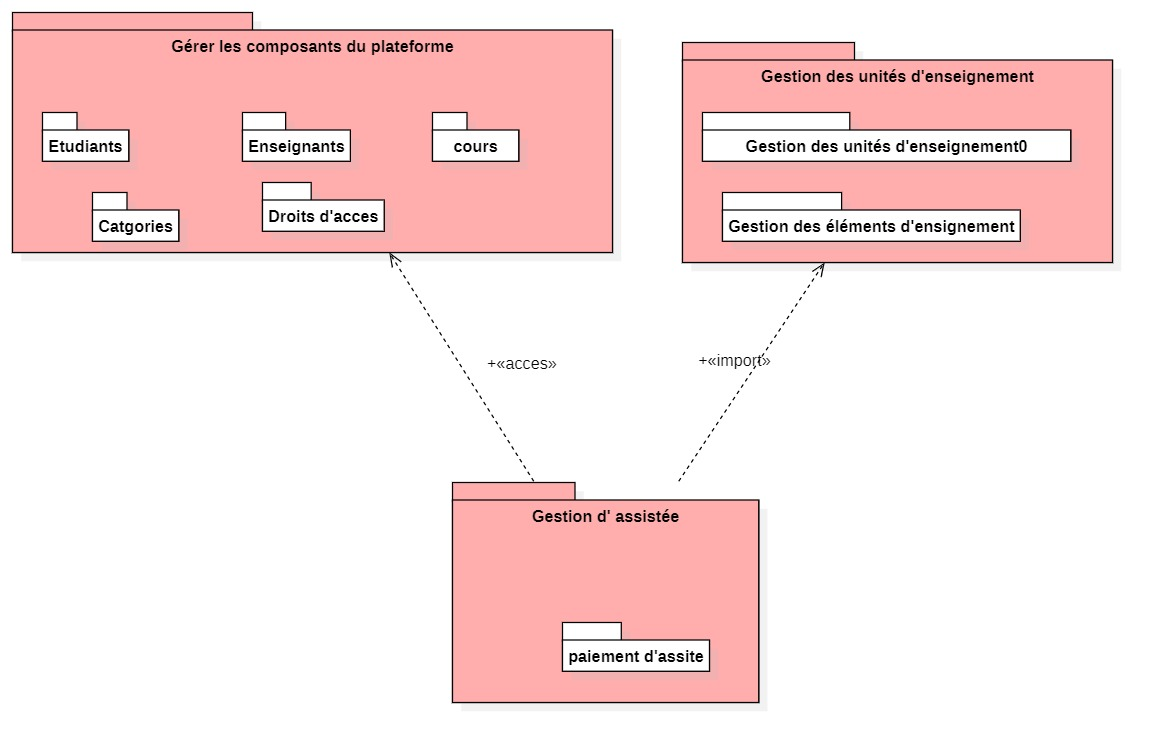
\includegraphics[width=18cm,height=10cm]{PackageDiagram1.jpg}
	\caption{Diagrammes de Package.}
	\label{fig:Diagrammes de Package}
\end{figure}
\FloatBarrier

    \section{ Etude d’enchainement des programmes}
Cette étape consiste à montrer les principaux modules développés pour la réalisation
d’une application.
Le menu général de notre application se présente selon le type de l’utilisateur.
\begin{figure}[ht]
	\centering
	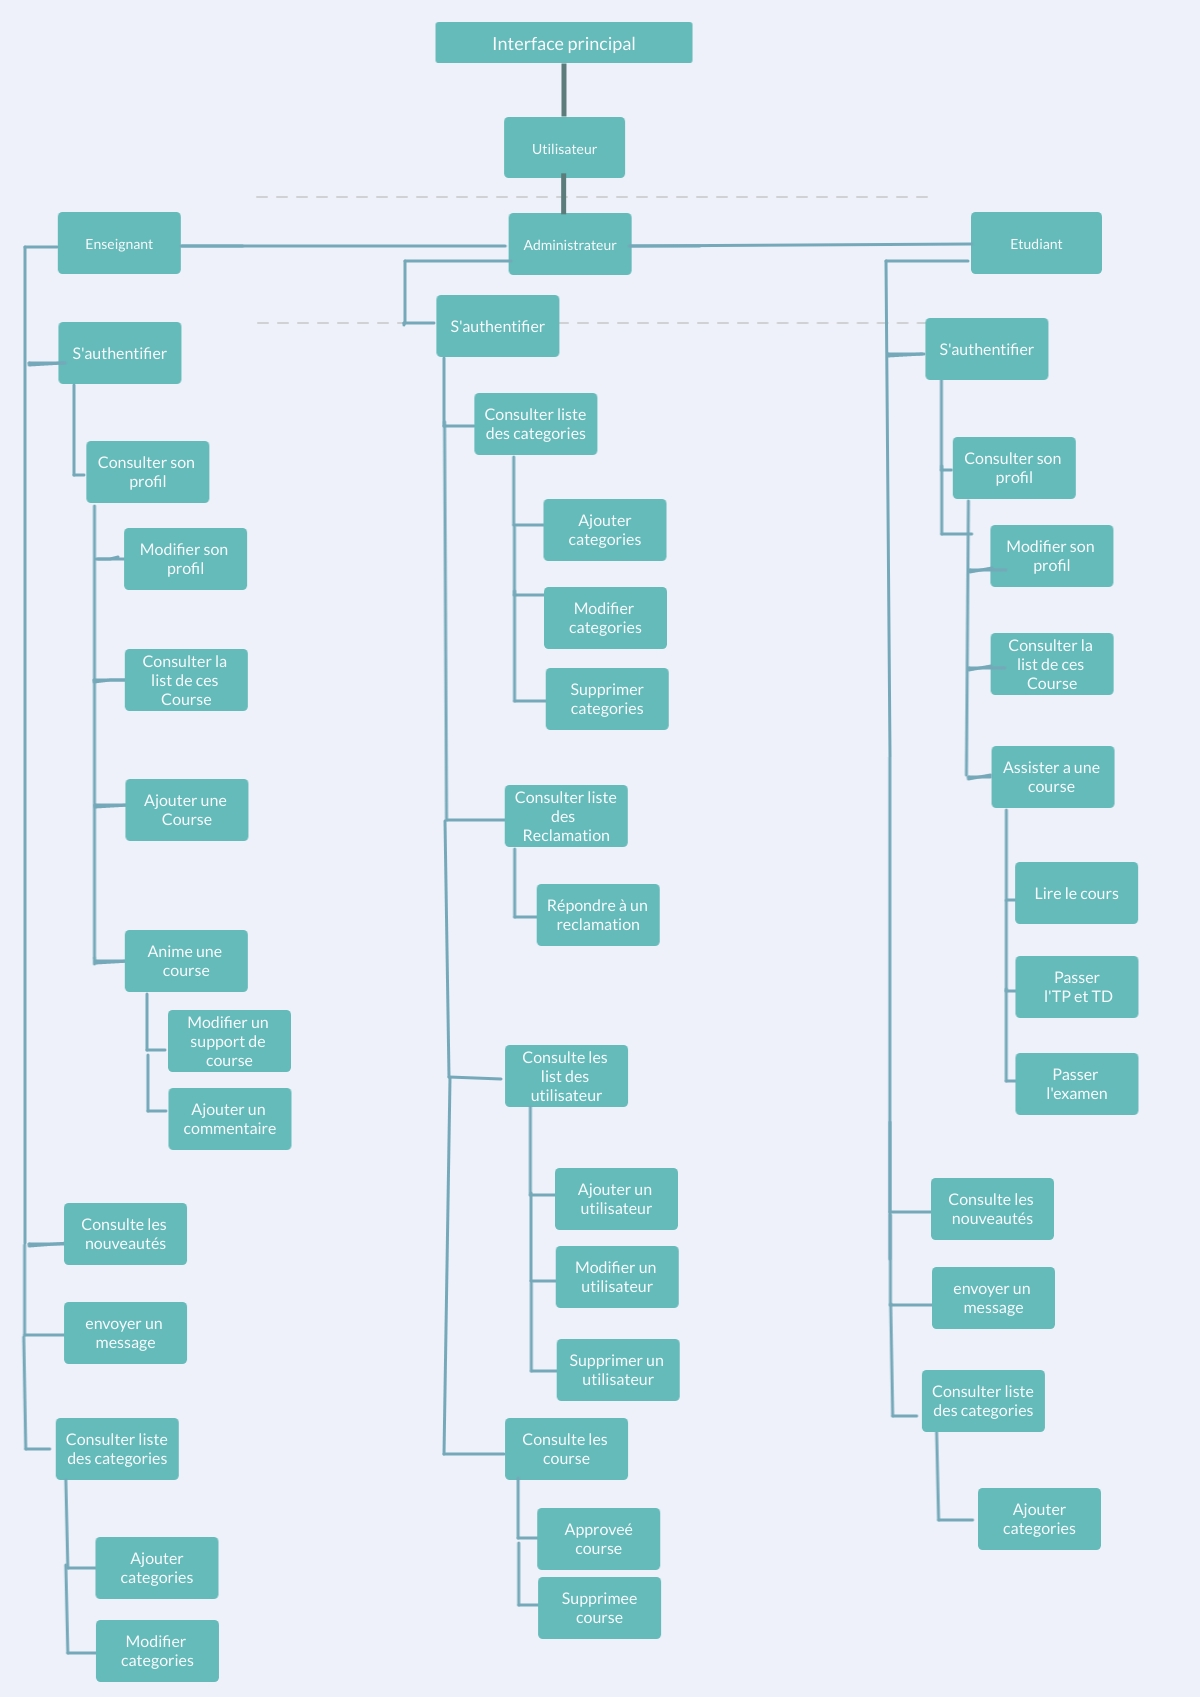
\includegraphics[width=18cm,height=16cm]{Untitled-Project.jpg}
	\caption{Enchainement des programmes.}
	\label{fig:enchainement des programmes}
\end{figure}
\FloatBarrier 

\section{Diagrammes des cas d'utilisation global}
Le modèle des cas d’utilisation décrit les fonctionnalités d’un système d’un point de vue utilisateur, sous la forme d’actions et de réactions ; l’ensemble des fonctionnalités est déterminé en examinant les besoins fonctionnels de tous les utilisateurs potentiels.\\
Ainsi, pour construire notre modèle, nous allons organiser les cas d’utilisation et les regrouper en ensembles fonctionnels cohérents. Pour ce faire, nous utilisons le concept général d’UML, le package.


Ce diagramme illustre le cas d’utilisation générale de notre système. Ces cas d’utilisation seront par la suite expliqués en détaille. (voir la figure \ref{fig:UseCaseAdmin}):
\begin{figure}[ht]
  \centering
  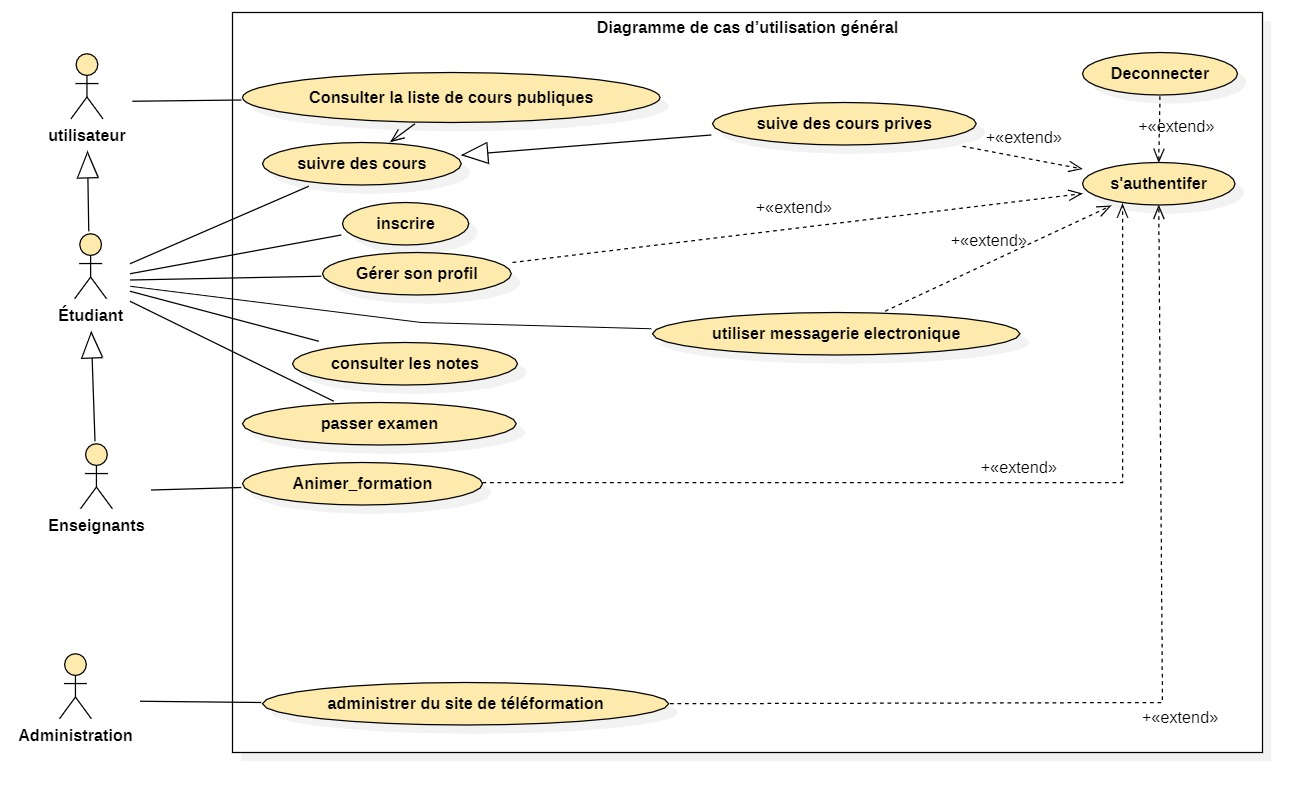
\includegraphics[width=18cm,height=14cm]{Diagrammedecasdutilisationgénéra.jpg}
  \caption{Les cas d'utilisation global.}
  \label{fig:UseCaseAdmin}
\end{figure}
\FloatBarrier


\section{Diagrammes de classes global}
Le diagramme de classes est un schéma utilisé en génie logiciel pour présenter les classes et les interfaces des systèmes ainsi que les différentes relations entre celles ci. Ce diagramme fait
partie de la partie statique d’UML car il fait abstraction des aspects temporels et dynamiques.
Une classe est un ensemble de fonctions et de données (attributs) qui sont liées ensembles par un champ sémantique . Dans ce qui suit nous allons décrire le diagramme de classes relatif à notre application.
 \ref{fig:UseCaseCatalogManager}. \\
 \\Voici quelques notions de base du diagramme :
  \begin{itemize}
 	\item \textit{\textbf{Une classe :}}  représente la description abstraite d'un ensemble d'objets
 	possédant les mêmes caractéristiques. On peut parler également de type. 
 	
 	\item \textit{\textbf{Un attribut :}} représente un type d'information contenu dans une classe .
 	
 	\item \textit{\textbf{Une opération  :}} représente un élément de comportement (un service)
 	contenu dans une classe.
 	
 
 	\item \textit{\textbf{Une association   :}} représente une relation sémantique durable entre deux
 	classes.
 	
 	\item \textit{\textbf{Une superclasse :}}
 	 est une classe plus générale reliée à une ou plusieurs
 	autres classes plus spécialisées (sous-classes) par une relation de
 	généralisation. Les sous-classes «Héritent» des propriétés de leur
 	superclasse et peuvent comporter des propriétés spécifiques
 	supplémentaires.
 	\end{itemize}
 \begin{figure}[ht]
 	\centering
 	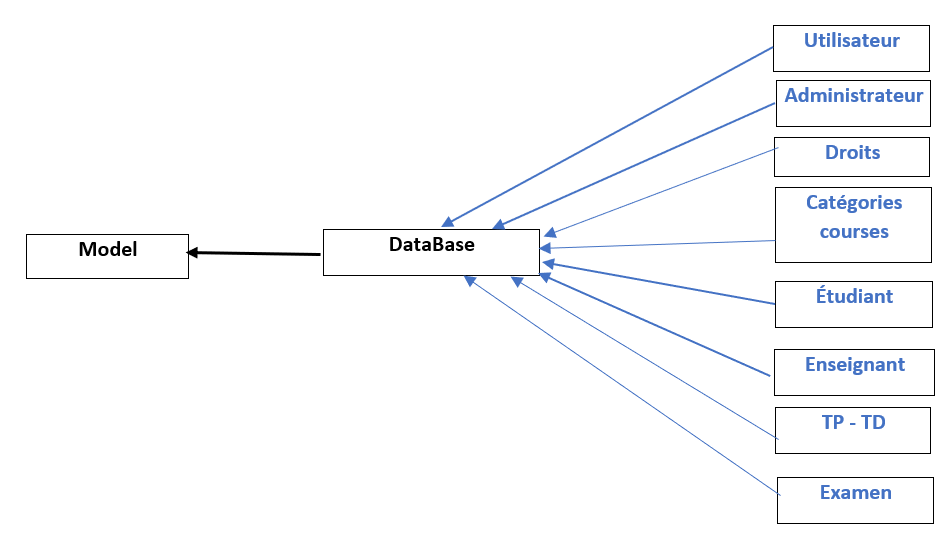
\includegraphics[width=13cm,height=6.80cm]{Larelation.jpg}
 	\caption{ La relation entre les différentes classes de l'application.}
 	\label{fig: La relation entre les différentes classes de l'application}
 \end{figure}
 \FloatBarrier
 \clearpage 
 La figure ci-dessous représente le diagramme de classes \cite{wiki:Diagramme_de_classes}:
 	
 
\begin{figure}[ht]
  \centering
  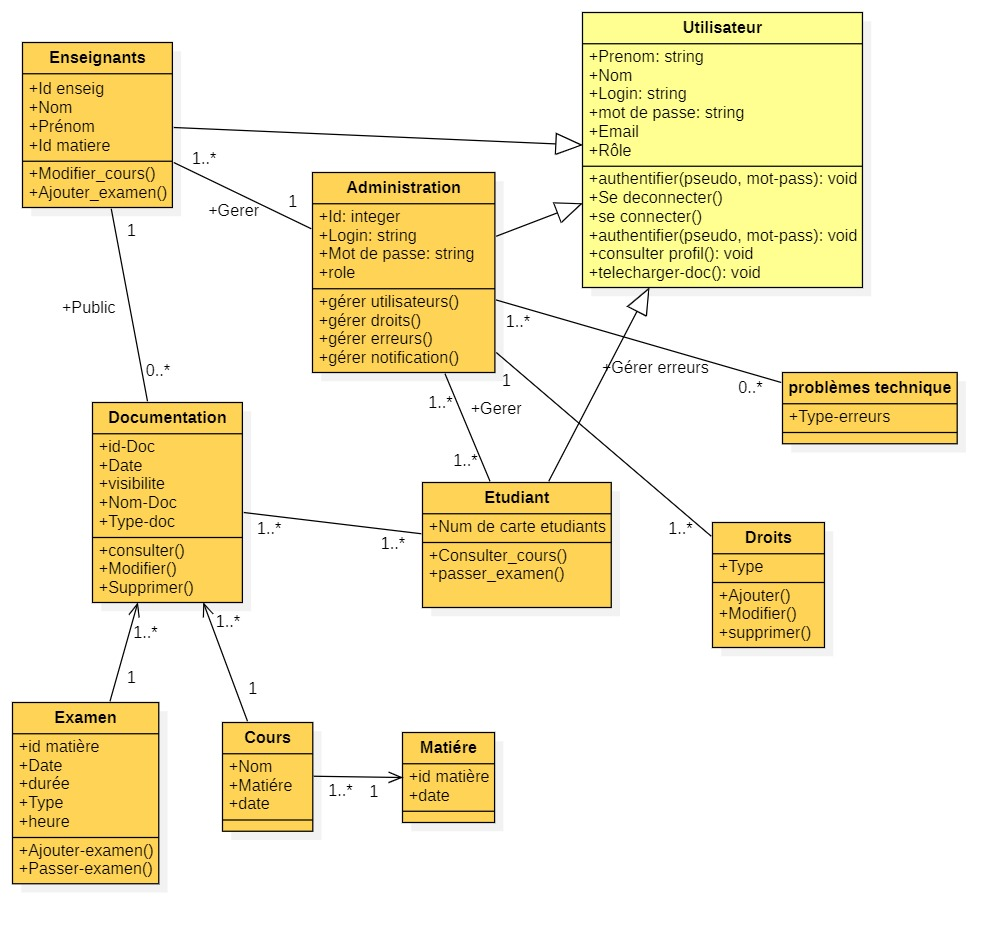
\includegraphics[width=18cm,height=16cm]{DiagrammedeclasseClassDiagram.jpg}
  \caption{Diagrammes de classes global.}
  \label{fig:UseCaseCatalogManager}
\end{figure}
\FloatBarrier
 \clearpage    

{\Large \color{cyan} Description des entités:}
 \smallskip
  \smallskip
   \smallskip
    \smallskip
     \smallskip
      \smallskip
       \smallskip
        \smallskip
         \smallskip
          \smallskip
           \smallskip
\begin{table}[h]
	\begin{itemize}
		
		\item \textit{\textbf{ Enseignants:}} L’utilisateur principal du module, il a accès à plusieurs fonctionnalités qui
		vont lui permettre de réussir le processus éducatif.
			\begin{itemize}	

			\item[$\star$] Faire un cours magistral :
			présentation, explication,
			argumentation et
			illustration d’un savoir
		


		\end{itemize}
	\end{itemize}
	\begin{center}
		\begin{tabular}{>{\begin{bf} } c <{\end{bf}}ccc}
			
			\rowcolor{-blue!20!red}Champs & \begin{bf}Types \end{bf} & \begin{bf}Contraintes\end{bf} & \\
			
			Id enseig & INT & PRIMARY KEY& \\
			
			Nom & VARCHAR(200)  & ---  &\\
			Prenom & VARCHAR(200)  & ---  &\\
			
			specialite  & VARCHAR & --- & \\
			specialite enseignement& INT& ---&\\

			email &VARCHAR(200)& UNIQUE&\\
telephone & VARCHAR(8) & ---& \\

			
		\end{tabular}
	\end{center}
	\caption{Tables  "Enseignants"}
	\label{Tables  "Enseignants"}
\end{table}
\smallskip
\smallskip
\smallskip
\begin{table}[h]
	
	\begin{itemize}
		
		\item \textit{\textbf{ Administration:}} On  le schéma de la base
		de données suivant :C'est la classe qui contient toutes les actions prises en charge
		par l'administrateur : 
	\end{itemize}
	\begin{center}
		\begin{tabular}{>{\begin{bf} } c <{\end{bf}}ccc}
			
			\rowcolor{-blue!20!red}Champs & \begin{bf}Types \end{bf} & \begin{bf}Contraintes\end{bf} & \\
			
			Id & INT & PRIMARY KEY& \\
			
			Nom &VARCHAR(200) & --- &\\
			prenom &VARCHAR(200) & --- &\\
			Mot de passe & VARCHAR(200)  & UNIQUE& \\
			
			role & VARCHAR(200) & UNIQUE  &\\
			email& VARCHAR(200)& UNIQUE &\\

		
			
		\end{tabular}
	\end{center}
	\caption{Tables  "Administration"}
	\label{mes belles tables}
\end{table}


\begin{table}[h]
	
	\begin{itemize}
		
		\item \textit{\textbf{ Etudiant:}} Le deuxième utilisateur du module avec des fonctionnalités facilitant la
		tâche de mémorisation.
	\end{itemize}
	\begin{center}
		\begin{tabular}{>{\begin{bf} } c <{\end{bf}}ccc}
			
			\rowcolor{-blue!20!red}Champs & \begin{bf}Types \end{bf} & \begin{bf}Contraintes\end{bf} & \\
			
			Num de carte etudiants & INT & PRIMARY KEY& \\
			nom & VARCHAR(200) & ---& \\
			prenom & VARCHAR(200) & ---& \\
			email &VARCHAR(200) &UNIQUE\\

			
			
			
			
		\end{tabular}
	\end{center}
	\caption{Tables  "Etudiant"}
	\label{mes belles table}
\end{table}

\begin{table}[h]
	
	\begin{itemize}
		
		\item \textit{\textbf{ TP/TD:}}C'est la classe qui contient toutes les TP et TD :
	\end{itemize}
	\begin{center}
		\begin{tabular}{>{\begin{bf} } c <{\end{bf}}ccc}
			
			\rowcolor{-blue!20!red}Champs & \begin{bf}Types \end{bf} & \begin{bf}Contraintes\end{bf} & \\
			
id &	INT(10)	&PRIMARY KEY& \\	
		\end{tabular}
	\end{center}
	\caption{Tables  "problèmes technique"}
	\label{Tables  "problèmes technique"s}
\end{table}














\begin{table}[h]
	
	\begin{itemize}
		
		\item \textit{\textbf{ Examen:}}  ça englobe toute les examens requis
	\end{itemize}
	\begin{center}
		\begin{tabular}{>{\begin{bf} } c <{\end{bf}}ccc}
			
			\rowcolor{-blue!20!red}Champs & \begin{bf}Types \end{bf} & \begin{bf}Contraintes\end{bf} & \\
			
			id &	INT(10)	&PRIMARY KEY& \\
			Date &VARCHAR(200) &---&\\
			durée & VARCHAR(200) &---&\\
			Type & VARCHAR(200) &---&\\
			heure & VARCHAR(200) &---&\\
			
		\end{tabular}
	\end{center}
	\caption{Tables  "Examen"}
	\label{Tables  "Examen"}
\end{table}










\begin{table}[h]
	
	\begin{itemize}
		
		\item \textit{\textbf{ Utilisateur:}}elle contient tous les utilisateurs du plateforme selon leur :
	\end{itemize}
	\begin{center}
		\begin{tabular}{>{\begin{bf} } c <{\end{bf}}ccc}
			
			\rowcolor{-blue!20!red}Champs & \begin{bf}Types \end{bf} & \begin{bf}Contraintes\end{bf} & \\
			id &INT &PRIMARY KEY&\\
pseudo& VARCHAR(200) &UNIQUE&\\
password& VARCHAR(200) &---&\\
privilege &VARCHAR(20) &---&\\


			
			
			
		\end{tabular}
	\end{center}
	\caption{Tables  "Utilisateur"}
	\label{Tables  "Utilisateur"}
\end{table}










\begin{table}[h]
	
	\begin{itemize}
		
		\item \textit{\textbf{ Cours:}}
	Toute les cours nécessaires au processus d'enseignement à distance
	\end{itemize}
	\begin{center}
		\begin{tabular}{>{\begin{bf} } c <{\end{bf}}ccc}
			
			\rowcolor{-blue!20!red}Champs & \begin{bf}Types \end{bf} & \begin{bf}Contraintes\end{bf} & \\

		id &	INT(10)	&PRIMARY KEY& \\
		
		user id&	INT(11)&---& \\
		
		category id&	INT(11)&---& \\
		
		title	&varchar(255)&---& \\	
		
		sub title&	varchar(255)&---& \\		
		
		description	&longtext	&---& \\
		
		about instructor&	longtext&---& \\	
		
		playlist url&	varchar(255)&---& \\	
		
		photo&	varchar(255)&---& \\	
		
		promo video url&	varchar(255)&---& \\	
		
		tags&	varchar(255)&---& \\	
		
		creator status&	INT(11)	&---& \\		
		
		admin status&	INT(11)	&---& \\	
		
		what will student learn&	longtext	&---& \\
		
		target student&	longtext&---& \\		
		
		requirements&	longtext&---& \\	
		
		discount price&	double(10,2)&---& \\		
		
		actual price&	double(10,2)	&---& \\	
		
		view count&	INT(11)	&---& \\		
		
		subscriber count&	int(11)	&---& \\
			
			
		\end{tabular}
	\end{center}
	\caption{Tables  "Cours"}
	\label{Tables  "Cours"}
\end{table}

\begin{table}[h]
    \begin{itemize}
      \item \textit{\textbf{ Catégorie Matiére:}}ca englobe toute les Matiéres
	\end{itemize}
	\begin{center}
		\begin{tabular}{>{\begin{bf} } c <{\end{bf}}ccc}
			
			\rowcolor{-blue!20!red}Champs & \begin{bf}Types \end{bf} & \begin{bf}Contraintes\end{bf} & \\
  

id 	&INT(10)	&PRIMARY KEY& \\	

name&	varchar(255)&---& \\	

description	&longtext&---	& \\

categories photos&	longtext&---& \\	

view count	&INT(11)&---	& \\		


			
			
		\end{tabular}
	\end{center}
	\caption{Tables  "Catégorie Matiére"}
	\label{Catégorie Matiére}
\end{table}
\clearpage 
\begin{table}[h]
	
	\begin{itemize}
		
		\item \textit{\textbf{ Droits:}}c'est la classe qui contient les droits attribués aux plateforme par
		l’administrateur ainsi la suppression ou l’ajout de certains privilèges.
	\end{itemize}
	\begin{center}
		\begin{tabular}{>{\begin{bf} } c <{\end{bf}}ccc}
			
			\rowcolor{-blue!20!red}Champs & \begin{bf}Types \end{bf} & \begin{bf}Contraintes\end{bf} & \\
			
			id & INT & PRIMARY KEY& \\
			titre & VARCHAR(200) & UNIQUE& \\
		\end{tabular}
	\end{center}
	\caption{Tables  "Droits"}
	\label{mTables  "Droits"}
\end{table}

\begin{table}[h]
	
	\begin{itemize}
		
		\item \textit{\textbf{ Email:}}c'est la classe qui contient tous les email des utilisateur .
	\end{itemize}
	\begin{center}
		\begin{tabular}{>{\begin{bf} } c <{\end{bf}}ccc}
			
			\rowcolor{-blue!20!red}Champs & \begin{bf}Types \end{bf} & \begin{bf}Contraintes\end{bf} & \\
			
			IdEmail & VARCHAR(50) & PRIMARY KEY& \\
			IdNom & VARCHAR(200) & ---& \\
		\end{tabular}
	\end{center}
	\caption{Tables  "Email"}
	\label{mTables  "Email"}
\end{table}
\begin{table}[h]
	
	\begin{itemize}
		
		\item \textit{\textbf{ Assister:}}c'est la classe qui contient les prix d'assister aux étudiant.
	\end{itemize}
	\begin{center}
		\begin{tabular}{>{\begin{bf} } c <{\end{bf}}ccc}
			
			\rowcolor{-blue!20!red}Champs & \begin{bf}Types \end{bf} & \begin{bf}Contraintes\end{bf} & \\
			
			Prix-assister & Float & PRIMARY KEY& \\
			
		\end{tabular}
	\end{center}
	\caption{Tables  "Assister"}
	\label{mTables  "Assister"}
\end{table}

\begin{table}[h]
	
	\begin{itemize}
		
		\item \textit{\textbf{ Note :}}c'est la classe qui contient les Notes des Etudiants
	\end{itemize}
	\begin{center}
		\begin{tabular}{>{\begin{bf} } c <{\end{bf}}ccc}
			
			\rowcolor{-blue!20!red}Champs & \begin{bf}Types \end{bf} & \begin{bf}Contraintes\end{bf} & \\
			
			Id-note & INT & PRIMARY KEY& \\
			Type-note & VARCHAR(200) & ---& \\
		\end{tabular}
	\end{center}
	\caption{Tables  "Note"}
	\label{mTables  "Note"}
\end{table}

\FloatBarrier

\section{Diagramme de déploiement}
Le Diagramme de déploiement représente l’architecture 3-tiers de notre application. La
Première partie représente l’utilisateur ainsi que son navigateur web. La partie serveur Web
représente le lieu de traitements des requêtes. La partie SGBD présente le systéme de gestion
de base de données "MySQL".
\begin{figure}[ht]
	\centering
	\includegraphics[width=18cm,height=8cm]{DiagrammedeDéploiement.png}
	\caption{Diagramme de déploiement.}
	\label{fig:Diagramme de déploiement}
\end{figure}
\FloatBarrier

\section{Conclusion}
Le but de ce chapitre était de définir et d’analyser l’ensemble des besoins fonctionnels  de notre solution. Cette étape est primordiale dans le développement d’un projet informatique puisque elle nous permet de définir le périmètre fonctionnel du projet, et de garantir la couverture de l’ensemble des fonctionnalités recensées.

\chapter{La réalisation}
\label{sec:conception}

\begin{fquote}Puisque Scrum est choisi comme méthode de gestion de projets, ce chapitre va être réparti selon
	les exigences de Scrum, en effet, le travail est divisé en Sprints, chacun d’eux a lieu de définir le but
	et le Sprint Backlog dans un premier temps, ensuite nous présentons la conception et la réalisation.
	Enfin, nous clôturons chaque Sprint par sa revue et une rétrospective.
 \end{fquote}

\clearpage

\section{Sprint 1 :}



\section{Conclusion}

Ce chapitre présente une vue conceptuelle de la solution à mettre en place. Il expose les différents diagrammes UML pour mieux comprendre les fonctionnalités offertes et pour mieux représenter la communication entre les différents objets du projet. Le chapitre suivant, présente la partie mise en œuvre de l’application.



\chapter{Mise en oeuvre de la solution}

\label{sec:realisation}

\begin{fquote}
Dans ce chapitre, on va présenter les outils utilisés pour la mise en oeuvre de la solution PIM ainsi qu’un aperçu des différentes vues et interfaces de cette solution.
\end{fquote}

\clearpage

\section{Introduction :}

Une des étapes de la vie d’un projet, aussi importante que la conception, est l’implémentation.

\medskip

Cette étape constitue la phase d’achèvement et d’aboutissement du projet. Pour accomplir cette tâche avec succès il faut savoir utiliser les outils adéquats et nécessaires. Ce choix d’outils peut influencer la qualité du produit obtenu et donc nécessite une attention particulière et doit se baser sur les besoins du projet et le résultat escomptés.

\medskip

Ce chapitre présente l’environnement technique du travail ainsi que le choix pris en matière d’environnement logiciel. 

\section{Outils et technologies utilisées :}
\subsection{La plateforme Java EE}

Java EE ou Java Enterprise Edition (récemment renommée Jakarta EE) est une norme proposée par la société Oracle, portée par un consortium de sociétés internationales, visant à définir un standard de développement d’applications d’entreprises multi-niveaux\cite{wiki:java}.

\medskip

Cette plate-forme est fortement orientée serveur et dédiée au développement et à l’exécution d’applications distribuées. Elle permet la simplification du processus de développement. En effet, JEE simplifie le contrôle et la gestion des ressources système en fournissant des méthodes permettant de gérer les transactions et la mise en commun des ressources.


\subsection{La plateforme SAP Hybris}

Hybris est une solution e-commerce créée en Allemagne, en 1997. Dès le début, la solution a ciblé son développement sur le « \textit{e-commerce} », le « \textit{PIM étendu} » et le « \textit{multi canal} »\cite{wiki:hybris}.


\medskip

Alors que certaines solutions sont clairement bâties pour faire la partie Front (produire du HTML pour faire des sites web), Hybris pense que le coeur du sujet, c’est pas le front, c’est le catalogue. L’idée, est de se dire qu’entre l’ERP, le système d’information de l’entreprise, et les sites Front, il y a besoin d’un middleware\cite{wiki:hybris}.
\medskip

Ce référentiel sera souvent alimenté par un système de plus bas niveau (ERP ou équivalent). A partir de ce référentiel, l’autre axe clé de Hybris, c’est le multi canal. En effet, Hybris permet de publier de manière cohérente, vers les différents canaux de vente : Web, mobile, magasin, etc…
\medskip

La platforme SAP Hybris repose sur des standards ouverts, qui conjugue l’efficacité et l’extensibilité afin d’offrir des capacités infinies d’innovation et de devenir la plate-forme de commerce la plus performante du marché. Ainsi la platforme repose sur plusieurs outils et frameworks open source et standardisés parmi lesquels on trouve :

\begin{itemize}
\medskip
    \item[$\bullet$] \textbf{Le Framework Spring\footnote{\url{https://spring.io/}} :} Un framework libre fournit un modèle complet de programmation et de configuration pour les applications d’entreprise modernes basées sur JEE. Le framework s'appuie principalement sur les principes de l'IOC (Inversion of Control) et de MVC (Model View Controller) \cite{wiki:spring}.
    \medskip

    \item[$\bullet$] \textbf{Apache Tomcat\footnote{\url{http://tomcat.apache.org/}} :} C'est un conteneur web libre de servlets et JSP Java EE. Issu du projet Jakarta. Il incorpore également un serveur HTTP\cite{wiki:tomcat}.
    
    % , c’est un des nombreux projets de l’Apache Software Foundation. Il implémente les spécifications des servlets et des JSP du Java Community Process, et paramétrable par des fichiers XML et des propriétés, et inclut des outils pour la configuration et la gestion.
    \medskip

    \item[$\bullet$] \textbf{Apache Solr\footnote{\url{https://lucene.apache.org/solr/}} :} C'est le moteur de recherche et d’indexation de référence dans le monde du libre. Basé sur la librairie Lucene, il dispose de nombreuses fonctionnalités avancées comme la recherche par facettes, la suggestion orthographique et la recherche par similarité \cite{wiki:solr}.
    \medskip

    \item[$\bullet$] \textbf{ZK Framework\footnote{\url{https://www.zkoss.org/}} :} C'est un framework open source web 2.0, proposant une interaction utilisateur riche. ZK permet tout autant de définir rapidement des interfaces graphiques via une syntaxe XML ou un éditeur Wysiwyg qui permet de manipuler directement les objets en Java \cite{wiki:zk}.
    \medskip
    
    \item[$\bullet$] \textbf{Apache Ant\footnote{\url{https://ant.apache.org/}} :} Ant est un logiciel créé par la fondation Apache qui vise à automatiser les opérations répétitives du développement de logiciel telles que la compilation, la génération de documents ou l'archivage au format JAR, à l'instar des logiciels Make. Ant est écrit en Java et son nom est un acronyme pour « Another Neat Tool » \cite{wiki:ant}.
    

\end{itemize}

\medskip

La plateforme SAP Hybris dispose par défaut des espaces d'administration suivants :

\begin{itemize}
\medskip
    \item[$\bullet$] \textbf{Le Framework Backoffice :} C'est la nouvelle version de l'encien HMC (Hybris Management Console), une interface backend du système qui permet de gérer les utilisateurs, les marchés et leurs catalogues de produits et les différents types du systèmes, il permet les opérations de création, mise à jour, suppression et de recherche à travers des millions d’articles\cite{sap}.
    \medskip
    \item[$\bullet$] \textbf{HAC (Hybris Administration Console) :} C’est une interface backend du système, il permet d’effectuer des opérations d’administrations comme la supervision des performances système, la modification à chaud des paramètres généraux, l’administration du cache système, de session, d’accès au logs etc\cite{sap}.
\end{itemize}

\subsection{Outils de développement et de collaboration :}

\subsubsection{L'IDE IntelliJ IDEA :} Également appelé « IntelliJ », « IDEA » ou « IDJ » est un environnement de développement intégré de technologie Java destiné au développement de logiciels informatique. Il est développé par JetBrains\footnote{\url{https://www.jetbrains.com/idea/}} (anciennement « IntelliJ ») et disponible en deux versions, l'une communautaire, open source, sous licence Apache 2 et l'autre propriétaire, protégée par une licence commerciale \cite{wiki:intellij}.

\subsubsection{Le système de contrôle des versions GIT :} C'est un logiciel libre de gestion de versions, créé par Linus Torvalds(le créateur du noyau Linux), c’est un outil bas niveau, qui se veut simple et très performant, dont la principale tâche est de gérer l’évolution du contenu d’une arborescence. Il fonctionne en mode distribué avec un serveur distant\cite{wiki:git}.

\subsubsection{Atlassian JIRA :} C'est un système de suivi de bugs, un système de gestion des incidents, et un système de gestion de projets développé par Atlassian. Jira\footnote{\url{https://www.atlassian.com/software/jira}} n'est pas un acronyme mais une troncation par aphérèse de Gojira\cite{wiki:jira}.

\section{Quelques interfaces de la plate-forme}
Les différentes interfaces qu'on présentera par la suite sont basé sur des composants ou bien des widgets d'Hybris qu'ils ont été personnalisé et évolués selon le besoin de la plate-forme.

\subsection{La page de Login}
La figure \ref{fig:login}  représente la page de login des utilisateurs. Cette page est composée des éléments suivants:
\medskip
\begin{enumerate}
    \item Logo
    \smallskip
    \item Formulaire d'authentification
    \smallskip
    \item Liste des langues disponibles
\end{enumerate}
\medskip




\subsection{La Vue Administration}

La vue Administration regroupe toutes les opérations de gestion des entités du PIM qu'elle soient natives à hybris comme les cronjob, les employés, les catalogues etc... ou celles spécifiquement crées pour le projet.
\bigskip

Cette vue est présentée dans les deux figures \ref{fig:admin} \ref{fig:admin-category} est composé des éléments suivants :

\begin{enumerate}
    \item Le menu d'administration qui regroupe les élément administrable dans le site sous forme d'arbres.
    \medskip
    \item Le composant de recherche dans les éléments/types du menu d'administration.
    \medskip
    \item Le composant de recherche dans la liste des objets de l'élément/type sélectionné.
    \medskip
    \item La liste des objets disponibles pour l'élément/le type sélectionné.
    \medskip
    \item Le composant d'édition des informations de l'objet sélectionne dans la liste 4.
    \medskip
    \item Les icônes de déconnexion, langues, profiles et d'autres natives a Hybris. 
\end{enumerate}

Dans la figure \ref{fig:admin} le type \textbf{Réference} est sélectionné alors que dans la figure \ref{fig:admin-category} le type de catégorie \textbf{Communication Fonctionnality} est sélectionnée: 




\subsection{La Vue Catalogue}

La vue catalogue présenté dans la figure \ref{fig:ctalog} est une espace de gestion avancé des produits du catalogue, elle est principalement composée des éléments suivants :

\begin{enumerate}
    \item Les composants de filtrage selon les catégories et les filtres prédéfinis.
    \item Le composant de recherche des produits.
    \item La liste des produits recherchés.
    \item Le nom de la vue "Wfj Catalog".
    \item L'image et la présentation du produit sélectionné.
    \item Le composant d'édition avancé des information du produit sélectionné.
\end{enumerate}


\subsection{La Vue Catégories}

La vue catégories La vue categories présenté dans la figure \ref{fig:category-vue} est une perspective qui permet de : 

\begin{itemize}
    \item[$\bullet$] Gérer les cétgories existantes au sein du PIM.
    \medskip
    \item[$\bullet$] Gérer des produits sur une catégorie sélectionnée, ie :
    \begin{itemize}
    \smallskip
        \item Rechercher des produits.
        \smallskip
        \item Associer des produits à une catégorie.
    \end{itemize}
\end{itemize}


\subsection{La Vue Dashboard}

Le dashboard WFJ permet d’afficher des indicateurs de suivi (voir la figure \ref{fig:dashboard}):

\begin{itemize}
    \item Un dashboard par statut (Approval Status) qui permet de voir le statut des produits par catégories (collection de communication).
    \smallskip
    \item Un dashboard qui indique le nombre de produits créés sur les 12 derniers mois.
    \smallskip
    \item Un dashboard pour les traductions par langue qui indique les produits qui ne sont pas traduits.
    
\end{itemize}



 


\section{Conclusion}
Dans ce chapitre, on a présenté la réalisation qu'on a effectué, l’environnement de développement, les outils et technologies utilisés dans le projet ainsi qu'une description détaillée des différentes interfaces utilisateur de la plate-forme.



%
\chapter*{Conclusion générale et perspectives}
\addcontentsline{toc}{chapter}{Conclusion générale}
\markboth{Conclusion}{Conclusion}
\label{sec:conclusion}
Notre projet intitulé « Conception et réalisation d’une pateforme d’E-learning » consiste à la conception et la réalisation d’une plateforme web destiné pour l’apprentissage en ligne.
\medskip
Contrairement à la majorité des travaux existants sur le marché qui offrent des fonctionnalités
limités et nécessitent un effort de configuration considérable, nous avons réalisé un système
qui permet à la fois de gérer des formations, simuler un salon de formation virtuel, et donner la possibilité aux formateurs de guider leurs apprenants .
\medskip
En ce qui concerne la démarche, nous avons en premier lieu 
commencé  par comprendre le contexte général de notre application et identifier les différentes exigences de notre futur système. Nous avons préparé par la suite notre planning de travail en respectant les priorités de nos besoins suite à une discussion entre l'équipe du développement et le directeur du produit.Tout au long de notre cycle de développement nous avons couplé la méthodologie Scrum par une autre méthodologie agile . En deuxième lieu nous avons spécifié notre application pour
discerner les fonctionnalités .En troisième lieu, nous avons procédé à sa conception ainsi
qu’aux choix technologiques pour sa réalisation. Enfin, nous l’avons mise en œuvre.
	\begin{figure}[ht]
	\centering
	\includegraphics[width=7cm,height=4cm]{Processusactueldedéveloppement.png}
	\caption{Logo StarUML.}
	\label{fig:StarUML }
\end{figure}
\FloatBarrier
\medskip
En terme de perspectives, le projet dans sa version actuelle n’est pas encore achevé, on est actuellement en cours du personnalisation de l'extension backoffice pour facilité encore plus l'accès et la gestion des informations des produits. Les prochaines itération porteront toujours sur ce sujet en plus de l'évolution du processus d'éxport des produits pour qu'il soit beaucoup plus personnalisable par l'utilisateur.
\medskip
    

    

%%% Local Variables: 
%%% mode: latex
%%% TeX-master: "isae-report-template"
%%% End: 



\clearpage
\thispagestyle{empty}

%choix du style de la biblio

\renewcommand\bibname{Webographie}
\bibliographystyle{ieeetr}
% \bibliographystyle{plain}
\bibliography{references}

\end{document}